\documentclass[11pt,a4paper]{article}
\usepackage[T1]{fontenc}
\usepackage[utf8]{inputenc}
\usepackage[british]{babel}
\usepackage{lmodern,microtype,amsmath,amssymb,amsthm,mathtools}
\usepackage[margin=25mm]{geometry}
\usepackage{booktabs,array,graphicx,xcolor,enumitem,tabularx}
\usepackage{tikz}
\usetikzlibrary{arrows.meta,positioning,calc}
\definecolor{plum}{HTML}{704365}
\definecolor{teal}{HTML}{237D80}
\usepackage[colorlinks=true,linkcolor=plum,citecolor=teal,urlcolor=teal]{hyperref}
\hypersetup{pdftitle={Algebraic extinction in acyclic spreading models},pdfauthor={Anonymous},pdfsubject={Counterexamples, genericity and support-checkable repairs of an exponential-extinction conjecture},pdfkeywords={spreading models, algebraic extinction, acyclic graphs, Metzler matrices, tricritical point, SWIR}}
\usepackage{fancyhdr}
\pagestyle{fancy}\fancyhf{}
\fancyhead[L]{\small Algebraic extinction in acyclic spreading models}
\fancyfoot[C]{\thepage}
\setlength{\headheight}{14pt}
\setlength{\parskip}{4pt}
\setlist{itemsep=2pt,topsep=4pt}
\newtheorem{theorem}{Theorem}[section]
\newtheorem{lemma}[theorem]{Lemma}
\newtheorem{proposition}[theorem]{Proposition}
\newtheorem{corollary}[theorem]{Corollary}
\theoremstyle{definition}\newtheorem{definition}[theorem]{Definition}
\theoremstyle{remark}\newtheorem{remark}[theorem]{Remark}
\newcommand{\R}{\mathbb R}
\newcommand{\dd}{\,\mathrm d}
\newcommand{\one}{\mathbf 1}
\newcommand{\Vs}{\mathcal V}
\newcommand{\Ps}{\mathcal P}
\newcommand{\norm}[1]{\left\lVert#1\right\rVert}
\newcommand{\status}[1]{\textsf{\small[#1]}}
\DeclareMathOperator{\spec}{spec}
\title{Algebraic extinction in acyclic spreading models:\\
explicit counterexamples, genericity and support-checkable repairs}
\author{Anonymous}
\date{21 October 2026 \\ \small Version 1.0.0-candidate. DOI: \href{https://doi.org/10.5281/zenodo.23548109}{10.5281/zenodo.23548109}}
\begin{document}
\maketitle

\begin{abstract}
Chan, Crommelin and Mandjes conjectured that, in their class of
interaction-driven spreading models, every vanishing compartment decays
exponentially whenever two graphs built from the model are acyclic or
nearly so. An earlier Evidence Press release refuted this conjecture with a
four-compartment model decaying like $18/t^2$, proved four compartments
necessary, and gave a spectral repair; within the source's encoding of
recovery, a no-direct-infection SWIR-type submodel also admits a
counterexample. The mechanism is an endgame in which the effective
reproduction number of the active compartment tends to exactly one.
This paper adds the following. A four-compartment model in which
\emph{both} graphs are acyclic has an explicit trajectory with
$x(t)\sim\sqrt{3/8}\,t^{-3/2}$. With four compartments no tail is slower
than $t^{-3/2}$. Acyclic chains give tails $t^{-1-1/m}$, optimal within
models driven by one active catalyst. In those models algebraic
extinction needs initial data in a null set, and exponential decay
returns after a perturbation at a rate governed by a general slowing
law. In the chain, SWIR and hierarchy families the slow tails never
follow an outbreak peak. Conditions checkable from the coefficient supports or the rates
restore the conjectured conclusion, and an exploratory simulation shows
how finite populations cut the tail short.
\end{abstract}

\noindent\textbf{MSC 2020:} 34D05 (primary); 92D30, 34C60, 15B48, 92C42.\\
\noindent\textbf{Keywords:} compartmental models; algebraic decay;
directed acyclic graphs; Metzler matrices; tricritical point;
critical slowing down.

\section{The question in words}
\label{sec:intro}

\emph{Goal: say what is being asked, why the answer is not obvious, and
what this paper proves.}

\paragraph{The setting.}
In a compartmental model of an epidemic or a rumour, a closed population
is divided into compartments: for example, people who have not heard a
rumour, people who have heard it once, active spreaders, and people who
have stopped spreading. Individuals move between compartments only when
they meet someone; the person met (the \emph{catalyst} of the move) keeps
their own state. Chan, Crommelin and Mandjes~\cite{CCM} call this class
\emph{interaction-driven dispersion models}. It contains the classical
SIR model of Kermack and McKendrick~\cite{KermackMcKendrick} and the
Daley--Kendall and Maki--Thompson rumour models~\cite{DaleyKendall,MakiThompson}; spontaneous recovery is
included by writing a recovery rate $\gamma x$ as $\gamma x\sum_j y_j$,
a ``contact with anyone''~\cite[eq.~(8), p.~9]{CCM}.

Two directed graphs summarise a model. The \emph{transition graph}
records who can move where; the \emph{dependency graph} records whose
presence a compartment needs in order to empty. If the transition graph
has no cycles, every compartment settles to a limit. Some compartments,
such as the active spreaders, \emph{vanish}: their fraction tends to
zero. The question is \emph{how fast}. For SIR the answer is
exponential: the number of infectious people eventually halves at a
fixed rate. Chan, Crommelin and Mandjes proved that under their graph
conditions a vanishing compartment is integrable, which rules out a
$1/t$ tail, and they conjectured that the decay is always exponential.

\paragraph{Why the answer matters, and the picture behind it.}
Exponential fade-out is what modellers assume when they extrapolate a
declining incidence curve to an elimination date. In SIR it holds for a
simple reason. At the end of an outbreak the susceptible fraction has
\emph{overshot} the herd-immunity threshold, so the effective
reproduction number $R_{\mathrm{eff}}(\infty)$ is strictly below one,
and the infectious fraction decays like
$\exp\{-(1-R_{\mathrm{eff}}(\infty))\gamma t\}$~\cite{Hethcote,DiekmannHeesterbeekBritton}.
Algebraic extinction is what happens if the endgame lands
\emph{exactly} on $R_{\mathrm{eff}}=1$. Then the active compartment is
replenished as fast as it is removed, at leading order, and decay
proceeds only through slower, higher-order effects.
In our main example $R_{\mathrm{eff}}(t)$ tends to one from below,
\[
1-R_{\mathrm{eff}}(t)\sim\frac{9}{2t},
\]
and the activity decays like $t^{-3/2}$ (Section~\ref{sec:counterexample}).
The graphs cannot see this balance, because it is a statement about
limiting \emph{rates}, not about which contacts are possible.

\paragraph{What was already known.}
Conjecture~1 has already been refuted. An earlier Evidence Press
release~\cite{EPprior} (by the same publisher as this paper) gives a four-compartment model with
$I(t)\sim18/t^2$, whose dependency graph contains the cycle
$Y\to I\to Y$; it also proves that four compartments are necessary,
constructs $(m+2)$-compartment models with tails $t^{-m/(m-1)}$, classifies
its four-compartment model, and proves that the logarithmic decay rate
of the vanishing mass equals the spectral bound of the limiting
transverse Jacobian. Section~\ref{sec:discussion} states precisely
where the present paper overlaps with that release. Separately, the
mean-field generalised epidemic process of Janssen, M\"uller and
Stenull~\cite[Sec.~II]{Janssen}, called the SWIR model by Choi, Lee and
Kahng~\cite{ChoiLeeKahng}, adds a ``weakened'' stage between
susceptible and infectious. With recovery written as in the source, its
no-direct-infection submodel belongs to the conjectured class and
admits a tricritical-type triple zero, hence a $t^{-3/2}$ counterexample
(Section~\ref{sec:swir}). Its dependency graph has cycles, and its
trajectory is not explicit. The source
itself notes that integrable tails such as $1/t^2$ are not excluded by
its integrability theorem~\cite[p.~24]{CCM}.

\paragraph{What this paper adds.}
Table~\ref{tab:contributions} lists the results, marking those that
overlap with~\cite{EPprior}, where to find them,
and how each is established. The labels mean: \emph{proof}, a complete
written argument; \emph{exact}, a symbolic or exact-rational
computation reproduced by the package; \emph{numerical}, a
floating-point check; \emph{exploratory}, a simulation or heuristic
without proof; \emph{open}, not settled.

\begin{table}[ht]
\centering\small
\begin{tabularx}{\textwidth}{@{}p{4.2cm}X p{1.9cm}@{}}
\toprule
Result & Content & Status\\
\midrule
SWIR in class (\S\ref{sec:swir}) & A no-direct-infection SWIR/GEP submodel admits a tricritical-type triple zero, hence a $t^{-3/2}$ counterexample. & proof; exact\\
Theorem~\ref{thm:base} & Four-state model, both graphs acyclic, explicit trajectory, $x\sim\sqrt{3/8}\,t^{-3/2}$; derived, not guessed. & proof; exact\\
Example~\eqref{eq:doubleexample} & Same graphs, $x\sim4t^{-2}$, codimension one. & proof; exact\\
Theorem~\ref{thm:minimal} & Three compartments never suffice (as in~\cite{EPprior}, Thm~5). & proof\\
Theorem~\ref{thm:hierarchy} & Tails $t^{-1-1/m}$, every even $m$, both graphs acyclic; slower at each even $N$ than~\cite{EPprior}, Thm~2. & proof; exact\\
Proposition~\ref{prop:dimension} & For $\dot y=xHy$: zero order $\le2\lfloor N/2\rfloor-1$, sharp. & proof\\
Corollary~\ref{cor:fourslowest} & At $N=4$ with one vanishing state, $t^{-3/2}$ is the slowest tail. & proof\\
Theorem~\ref{thm:four} & Any $N=4$ model: exponential, $t^{-2}$ or $t^{-3/2}$; nothing slower. & proof; numerical examples\\
Theorem~\ref{thm:classification} & All rates and data of the four-state chain: exponential, $t^{-2}$ or $t^{-3/2}$. & proof\\
Theorem~\ref{thm:generic} & Algebraic extinction is confined to a null set of data for $\dot y=xHy$; codimensions 1 and 2 in the chain. & proof; exact\\
Theorem~\ref{thm:slowing} & Order-$k$ zero: perturbed rate $\propto|\varepsilon|^{(k-1)/k}$, endpoint shift $\propto|\varepsilon|^{1/k}$, jump for even $k$. & proof; numerical\\
Proposition~\ref{prop:nopeak} & No outbreak peak precedes an algebraic tail in the chain, SWIR and hierarchy families. & proof; exact\\
Theorem~\ref{thm:spectral} & Logarithmic rate equals $s(J)$ of the limiting Metzler block (same statement as~\cite{EPprior}, Thm~7, Cor.~8). & proof\\
Corollary~\ref{cor:graph} & Support-checkable condition for exponential extinction. & proof\\
Corollary~\ref{cor:rates} & Rate-checkable condition; rates alone cannot decide a trajectory's tail. & proof\\
Section~\ref{sec:finite} & Finite populations: extinction at $\approx1.5N^{0.42}$. & exploratory\\
\bottomrule
\end{tabularx}
\caption{Results and their status.}
\label{tab:contributions}
\end{table}

\paragraph{Roadmap.}
Section~\ref{sec:model} sets out the model, quotes the source's
hypotheses verbatim, and introduces the two clocks used throughout.
Section~\ref{sec:counterexample} derives the explicit counterexample,
checks it against each hypothesis, and gives the $t^{-2}$ and SWIR
examples. Section~\ref{sec:minimality} proves minimality.
Section~\ref{sec:hierarchy} gives the hierarchy, the dimension bound and
the slowest four-compartment tail.
Section~\ref{sec:chain} analyses the four-state chain completely:
classification, genericity, the slowing law and the absence of a peak.
Section~\ref{sec:spectral} gives the limiting-block criterion and the
support- and rate-checkable repairs. Section~\ref{sec:finite} discusses
finite populations, and Section~\ref{sec:discussion} the literature and
open problems. Readers who want only the disproof need
Sections~\ref{sec:model} and~\ref{sec:counterexample}.

\paragraph{Notation.} Table~\ref{tab:notation} fixes the symbols; each
is used in one sense only.

\begin{table}[ht]
\centering\small
\begin{tabularx}{\textwidth}{@{}lX@{}}
\toprule
Symbol & Meaning\\
\midrule
$N$, $y_i$, $y^*$ & number of compartments; fraction in compartment $i$; limit of $y(t)$\\
$c_{ijk}$, $\beta^j_{ik}$ & contact coefficient (donor $i$, destination $j$, catalyst $k$); source notation, $c_{ijk}=\beta^j_{ik}$\\
$\varphi_{ijk}$ & flux $c_{ijk}y_iy_k$\\
$\Vs,\Ps$ & vanishing and persistent compartments ($y_i^*=0$, resp.\ $>0$)\\
$x$ & fraction in the active compartment $X$\\
$u(t)$, $U$ & exposure clock $\int_0^tx$; its limit $u(\infty)$\\
$\Phi(u)$ & active fraction as a function of exposure, $x(t)=\Phi(u(t))$\\
$s,w,x,r$ & fractions in the base chain $S\to W\to X\to R$\\
$\vartheta(t)$, $\zeta(t)$ & $\vartheta=(16+2t/3)^{-1/2}$, $\zeta=1+\vartheta$ (base chain)\\
$\alpha,\beta,\gamma$ & rates of the general four-state chain\\
$q$, $Q(q)$, $q_*$ & $q=e^{-u}$; exposure cubic for rates $(2,1,1)$; its attained root\\
$\kappa$ & second exposure derivative at a double zero\\
$\nu,\eta$ & SWIR rates $S\to W$ and $W\to I$ (recovery rate $1$)\\
$m$, $w_k$, $\varrho$ & hierarchy order, reservoir fractions, $\varrho=1/(m+1)$\\
$H$, $k$, $a_k$ & matrix in $\dot y=xHy$; order of the first zero of $\Phi$; $\Phi(U-v)=a_kv^k+\dots$\\
$M_N$ & $2\lfloor N/2\rfloor-1$\\
$J$, $s(J)$ & limiting Metzler block of the vanishing coordinates; spectral abscissa\\
$\varepsilon$, $\delta$, $\Gamma$ & perturbation size and direction; induced profile change $\Gamma(u)$\\
$\omega$ & an exponential decay rate\\
\bottomrule
\end{tabularx}
\caption{Notation.}
\label{tab:notation}
\end{table}

\section{Model, the source's hypotheses, and two clocks}
\label{sec:model}

\emph{Goal: state the class exactly as the source does, so that every
later verification can be checked line by line.}

\subsection{The model}
There are $N$ fractions $y_i>0$ with $\sum_iy_i=1$. For a donor $i$, a
destination $j\ne i$ and a catalyst $k$ (which may equal $i$ or $j$) let
$c_{ijk}\ge0$ be constant. The flux $\varphi_{ijk}=c_{ijk}y_iy_k$ moves
mass from $i$ to $j$, and
\begin{equation}
\dot y_i=\sum_{a\ne i}\sum_{k}c_{aik}\,y_ay_k
        -y_i\sum_{b\ne i}\sum_kc_{ibk}\,y_k .
\label{eq:model}
\end{equation}
In the source notation $c_{ijk}=\beta^j_{ik}$ for $j\ne i$ and
$\beta^i_{ik}=\sum_{j\ne i}c_{ijk}$, which is the source's conservation
law~\cite[eq.~(2), p.~7]{CCM}; \eqref{eq:model} is then the source's
system~\cite[eqs.~(1)--(4), pp.~6--7]{CCM}. The simplex is invariant,
$\dot y_i\ge-C_iy_i$ for a constant $C_i$, so positive coordinates stay
positive at finite times, and solutions are global.

\subsection{The hypotheses, quoted}
\label{sec:quotes}
Page numbers refer to the PDF of arXiv:2511.02437v1 (only version
1 exists at the time of writing); the file's SHA-256 is recorded in the
package.
\begin{itemize}
\item Initial data~\cite[p.~6]{CCM}: ``Initial conditions are assumed to
be $y_i(0)\in(0,1)$.''
\item Transition graph, Definition~6~\cite[p.~7]{CCM}: ``The set of
directed edges $E$ contains an edge $(u,v)\in V\times V$ with $u\ne v$
if and only if there exists some state $k\in V$ such that
$\beta^v_{uk}>0$.''
\item Dependency graph, Definition~7~\cite[p.~8]{CCM}: ``The set of
directed edges $E$ contains an edge $(u,v)\in V\times V$ if and only if
$\beta^u_{uv}>0$.'' And: ``(Self-loops $i\to i$ occur when
$\beta^i_{ii}>0$.)''
\item Assumption~1~\cite[p.~11]{CCM}: ``The underlying transition graph
of the interaction-driven dispersion model is a DAG.''
\item Definition~8~\cite[p.~14]{CCM}: ``We call state $i$ vanishing if
$\lim_{t\to\infty}y_i(t)=0$ and persistent if
$\lim_{t\to\infty}y_i(t)>0$.''
\item Assumption~2~\cite[p.~15]{CCM}: ``Every cycle in the underlying
dependency graph contains at least one state with a persistent
dependency successor.''
\item Meaning of exponential decay~\cite[§3.3, p.~24]{CCM}: ``there
exist constants $C>0$ and $r>0$ such that $y_i(t)\le Ce^{-rt}$.''
\item Conjecture~1~\cite[p.~25]{CCM}: ``Under Assumption 1 and 2,
every vanishing state decays exponentially to 0.''
\end{itemize}
In our notation: the transition graph has an edge $i\to j$ iff
$c_{ijk}>0$ for some $k$; the dependency graph has an edge $i\to k$ iff
$c_{ijk}>0$ for some $j$ (donor to catalyst, self-loops allowed when
$k=i$). We write (G1) for Assumption~1 and (G2) for Assumption~2.
Persistence is judged by limits, as in Definition~8, so (G2) refers to
labels of the trajectory. The source's Corollary~1~\cite[p.~22]{CCM}
reads: ``Under Assumptions 1 and 2, if the persistent successor within
each cycle of the dependency graph is identifiable, then the asymptotic
characterization of every state can be determined.'' It adds that this
characterization depends ``only on whether each $\beta$-coefficient is
zero or non-zero''. So, when that identifiability condition holds, the
labels are determined by the supports of the coefficients.
The conjecture has no genericity clause: one trajectory suffices to
refute it. Our explicit counterexamples have acyclic graphs without
self-loops under either orientation of the dependency edges, so they do
not depend on this convention. The minimality theorem
(Section~\ref{sec:minimality}) uses the orientation above, which is the
source's.

\subsection{Two facts and two clocks}

\begin{lemma}[Finite total flux under (G1)]
\label{lem:flux}
Under (G1), every coordinate has a limit $y_i^*$, every flux is
integrable on $[0,\infty)$ and tends to zero, and
\begin{equation}
c_{ijk}>0\ \Longrightarrow\ y_i^*y_k^*=0.
\label{eq:fluxzero}
\end{equation}
\end{lemma}
\begin{proof}
Label compartments topologically, so $c_{ijk}>0$ implies $i<j$. The
bounded function $L=\sum_i iy_i$ has
$\dot L=\sum(j-i)\varphi_{ijk}\ge\sum\varphi_{ijk}\ge0$, because
$j-i\ge1$. Hence the total flux is integrable, so is each
$|\dot y_i|$, and each coordinate converges. Each flux then has a
limit, which is zero because the flux is integrable.
\end{proof}

\begin{lemma}[Integrability and persistent successors]
\label{lem:integrability}
Under (G1)--(G2), every vanishing coordinate is integrable and has a
persistent dependency successor, and every dependency successor of a
persistent state vanishes.
\end{lemma}
\begin{proof}
A state $i$ with a persistent dependency successor $k$ is integrable:
some outflow $c_{ijk}y_iy_k$ is eventually at least
$\tfrac12c_{ijk}y_k^*\,y_i$ and is integrable by Lemma~\ref{lem:flux}.
Let $B$ be the set of vanishing, non-integrable states and suppose
$B\ne\varnothing$. By the previous sentence no member of $B$ has a
persistent dependency successor. Since
$y_i(t)\ge y_i(0)\exp(-\int_0^th_i)$ with per-capita outflow
$h_i=\sum_{j,k}c_{ijk}y_k$, a vanishing $i$ has $\int_0^\infty h_i=\infty$,
so some dependency successor of $i$ is non-integrable. That successor
is not persistent (persistent states are not integrable), and it is not
integrable, so it lies in $B$. Following successors inside the finite
set $B$ produces a cycle in $B$, and (G2) gives one of its vertices a
persistent successor: a contradiction. Thus $B=\varnothing$. If a
vanishing state had only vanishing successors, all would be integrable,
its integrated hazard would be finite, and it could not vanish.
Finally a persistent state cannot have a persistent successor
by~\eqref{eq:fluxzero}.
\end{proof}
Both lemmas restate results of the source~\cite[Theorem~2, p.~17;
Theorem~3, p.~19]{CCM}; we include proofs because later arguments use
their internal steps.

\paragraph{Two clocks.}
Ordinary time $t$ is the clock in which we measure decay. The
\emph{exposure clock} is the cumulative activity
\[
u(t)=\int_0^tx(\sigma)\dd\sigma,
\]
the total amount of contact with the active compartment up to time $t$.
When every flux has the active fraction $x$ as a factor, dividing by
$\dot u=x$ makes the equations \emph{linear} in $u$; this is the
device behind Kermack and McKendrick's final-size
equation~\cite{KermackMcKendrick} and its use in rumour
models~\cite{Arruda,Rada}. In exposure time everything is explicit.
The only nonlinear step is to convert back to $t$ through the scalar
equation $\dot u=\Phi(u)$, where $\Phi(u)$ is the active fraction at
exposure $u$. The total exposure $U=u(\infty)$ is finite exactly when
$x$ is integrable, and then $x(t)\to0$ at a rate set by how $\Phi$
vanishes at $U$: a simple zero gives exponential decay, and a zero of
order $k\ge2$ gives $t^{-k/(k-1)}$. Exponential decay versus a power law
is therefore a question about the multiplicity of one zero of an
explicit function. In dynamical-systems terms the endpoint is a
non-hyperbolic boundary equilibrium, and the slow tail is an approach
along a centre direction~\cite{Carr}; what is at issue is whether that
approach is compatible with the source's graph conditions.

\section{The counterexample, derived}
\label{sec:counterexample}

\emph{Goal: construct an explicit trajectory that satisfies every
hypothesis of the conjecture and still decays like $t^{-3/2}$, showing
where the numbers come from.}

\subsection{A staged rumour with stifling}

Take four compartments: $S$ (unaware), $W$ (primed: heard once), $X$
(active spreader) and $R$ (stifler), with fractions $s,w,x,r$. There
are three contact moves, shown in Figure~\ref{fig:diagram}: an unaware
person who meets a spreader becomes primed (rate $2$); a primed person
who meets a spreader becomes a spreader (rate $1$); a spreader who
meets a stifler stops spreading (rate $1$). In the source's notation
the only nonzero coefficients are
\[
\beta^W_{SX}=2,\qquad \beta^X_{WX}=1,\qquad \beta^R_{XR}=1,
\]
and the equations are
\begin{equation}
\dot s=-2sx,\qquad \dot w=2sx-wx,\qquad \dot x=(w-r)x,\qquad \dot r=rx.
\label{eq:base}
\end{equation}
This is a two-step version of the rumour-scotching model of de Arruda
et al.~\cite[eq.~(3.2)]{Arruda}, close to the repetition models of Rada
et al.~\cite{Rada}. In this model the effective reproduction number of
the spreaders is $R_{\mathrm{eff}}=w/r$, the ratio of their
per-capita production and removal rates.

\begin{figure}[ht]
\centering
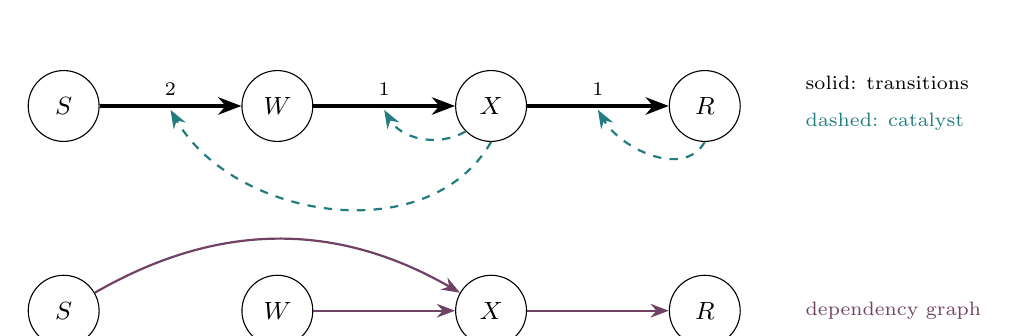
\begin{tikzpicture}[>=Stealth, node distance=18mm,
  st/.style={draw,circle,minimum size=9mm,font=\small},
  cat/.style={->,dashed,teal,thick}]
\node[st] (S) {$S$};
\node[st,right=of S] (W) {$W$};
\node[st,right=of W] (X) {$X$};
\node[st,right=of X] (R) {$R$};
\draw[->,very thick] (S) -- node[above,font=\scriptsize]{$2$} (W);
\draw[->,very thick] (W) -- node[above,font=\scriptsize]{$1$} (X);
\draw[->,very thick] (X) -- node[above,font=\scriptsize]{$1$} (R);
\draw[cat] (X.south) to[out=-120,in=-60] ($(S)!0.5!(W)+(0,-0.05)$);
\draw[cat] (X.south west) to[out=-150,in=-60] ($(W)!0.5!(X)+(0,-0.05)$);
\draw[cat] (R.south) to[out=-120,in=-60] ($(X)!0.5!(R)+(0,-0.05)$);
\node[font=\scriptsize,align=left,anchor=west] at (9.3,0.3) {solid: transitions};
\node[font=\scriptsize,align=left,anchor=west,teal] at (9.3,-0.2) {dashed: catalyst};
\begin{scope}[yshift=-2.6cm]
\node[st] (S2) {$S$};
\node[st,right=of S2] (W2) {$W$};
\node[st,right=of W2] (X2) {$X$};
\node[st,right=of X2] (R2) {$R$};
\draw[->,thick,plum] (S2) to[bend left=30] (X2);
\draw[->,thick,plum] (W2) -- (X2);
\draw[->,thick,plum] (X2) -- (R2);
\node[font=\scriptsize,anchor=west,plum] at (9.3,0) {dependency graph};
\end{scope}
\end{tikzpicture}
\caption{The base chain. Top: transition graph (solid) with the catalyst
of each move (dashed); the transition graph is the path
$S\to W\to X\to R$. Bottom: the dependency graph, with edges from each
donor to the catalyst of its outflow. Both graphs are acyclic and have
no self-loops. Note that $W\to X$ is catalysed by its own destination
$X$; this autocatalytic inflow is invisible to the dependency graph and
is the source of the slow tail (Section~\ref{sec:spectral}).}
\label{fig:diagram}
\end{figure}

\subsection{Finding the trajectory}
Every flux in~\eqref{eq:base} contains $x$, so in the exposure clock
$u$ the system is linear: $s'=-2s$, $w'=2s-w$, $r'=r$ (primes denote
$\dd/\dd u$). With $q=e^{-u}$ and initial data $(s_0,w_0,x_0,r_0)$,
\[
s=s_0q^2,\qquad w=(w_0+2s_0)q-2s_0q^2,\qquad r=\frac{r_0}q,\qquad
x=1-s-w-r=\frac{Q(q)}q,
\]
with the \emph{exposure cubic}
\begin{equation}
Q(q)=s_0q^3-(w_0+2s_0)q^2+q-r_0 .
\label{eq:cubic}
\end{equation}
Since $\dot q=-qx=-Q(q)$, the activity vanishes when $q$ reaches the
largest root $q_*\in(0,1)$ of $Q$ (note $Q(0)=-r_0<0<x_0=Q(1)$). A simple
root gives exponential decay. To make the decay as slow as possible we
ask for a triple root, $Q(q)=s_0(q-q_*)^3$. Matching coefficients gives
\begin{equation}
s_0=\frac1{3q_*^2},\qquad w_0=\frac{3q_*-2}{3q_*^2},\qquad
r_0=\frac{q_*}3,\qquad x_0=\frac{(1-q_*)^3}{3q_*^2},
\label{eq:triplefamily}
\end{equation}
which is positive exactly for $2/3<q_*<1$. Then
$\dot q=-s_0(q-q_*)^3$, and $\vartheta=q/q_*-1$ solves
$\dot\vartheta=-\vartheta^3/3$. The choice $q_*=4/5$ gives rational data
and $\vartheta(0)=1/4$.

\begin{theorem}[Explicit counterexample with both graphs acyclic]
\label{thm:base}
Let $\vartheta(t)=(16+\tfrac23t)^{-1/2}$ and $\zeta=1+\vartheta$. The
solution of~\eqref{eq:base} with
\begin{equation}
(s_0,w_0,x_0,r_0)=\Bigl(\frac{25}{48},\frac5{24},\frac1{240},\frac4{15}\Bigr)
\label{eq:baseinitial}
\end{equation}
is
\begin{equation}
s=\frac{\zeta^2}3,\qquad w=\frac{\zeta(3-2\zeta)}3,\qquad
x=\frac{\vartheta^3}{3\zeta},\qquad r=\frac1{3\zeta}.
\label{eq:base_trajectory}
\end{equation}
It is strictly positive, tends to $(1/3,1/3,0,1/3)$, and
\begin{equation}
x(t)\sim\sqrt{3/8}\;t^{-3/2},\qquad
\int_0^\infty x(t)\dd t=\log\frac54 .
\label{eq:baseresult}
\end{equation}
Every hypothesis of Conjecture~1 holds, so the conjecture is false
even when the dependency graph is also acyclic.
\end{theorem}

\begin{proof}
With $q_*=4/5$,~\eqref{eq:triplefamily} gives~\eqref{eq:baseinitial},
and $\zeta=q/q_*$. Substituting $q=\tfrac45\zeta$ in the exposure
formulas gives~\eqref{eq:base_trajectory}; the identity
$1+\vartheta^3=\zeta(\zeta^2-3\zeta+3)$ confirms that the four
fractions sum to one. Since $0<\vartheta\le1/4$ we have
$1<\zeta\le5/4$ and $3-2\zeta\ge1/2$, so all fractions are positive.
As $t\to\infty$, $\vartheta\to0$, which gives the limit, and
$x\sim\tfrac13(\tfrac32)^{3/2}t^{-3/2}=\sqrt{3/8}\,t^{-3/2}$. The total
exposure is $u(\infty)=\log(1/q_*)=\log(5/4)$. A power law excludes any
bound $Ce^{-rt}$, so $x$ is a vanishing state without exponential
decay. The hypothesis check is Table~\ref{tab:hypcheck}.
\end{proof}

\begin{table}[ht]
\centering\small
\begin{tabularx}{\textwidth}{@{}p{3.6cm}X@{}}
\toprule
Source hypothesis & Check for~\eqref{eq:base}--\eqref{eq:baseinitial}\\
\midrule
$y_i(0)\in(0,1)$ (p.~6) & $25/48,5/24,1/240,4/15$ lie in $(0,1)$ and sum to one.\\
Model (1)--(4), conservation (2) (pp.~6--7) & Coefficients constant and nonnegative; $\beta^S_{SX}=\beta^W_{SX}=2$, $\beta^W_{WX}=\beta^X_{WX}=1$, $\beta^X_{XR}=\beta^R_{XR}=1$, all others zero.\\
Def.~6 transition graph (p.~7) & Edges $S\to W$, $W\to X$, $X\to R$: a path.\\
Assumption~1 (p.~11) & The path is a DAG.\\
Def.~7 dependency graph (p.~8) & $\beta^u_{uv}>0$ only for $(S,X)$, $(W,X)$, $(X,R)$; no self-loops since $\beta^i_{ii}=0$ for all $i$.\\
Assumption~2 (p.~15) & The dependency graph has no cycle, so the condition holds vacuously (the source notes it ``is met by any DAG'', p.~15).\\
Def.~8 labels (p.~14) & $S,W,R$ persistent ($\to1/3$), $X$ vanishing.\\
Exponential decay (p.~24) & Fails: $x(t)\,e^{\epsilon t}\to\infty$ for every $\epsilon>0$.\\
\bottomrule
\end{tabularx}
\caption{Hypothesis-by-hypothesis check against the source, with page
pinpoints from Section~\ref{sec:quotes}.}
\label{tab:hypcheck}
\end{table}

\paragraph{The balance in words.}
Along the trajectory
$R_{\mathrm{eff}}=w/r=\zeta^2(3-2\zeta)$, so
\[
1-R_{\mathrm{eff}}=(\zeta-1)^2(2\zeta+1)\sim\frac9{2t},\qquad
\frac{\dot x}x=w-r=-r(1-R_{\mathrm{eff}})\sim-\frac3{2t},
\]
which is the exponent $3/2$. Heuristically, a tail $t^{-\theta}$ corresponds
to $1-R_{\mathrm{eff}}(t)\approx\theta/(\gamma r^*t)$, where $\gamma r^*$
is the limiting per-capita removal rate.

\paragraph{How tuned is this?}
The data~\eqref{eq:baseinitial} are tuned: at fixed rates the
$t^{-3/2}$ trajectories form the one-parameter curve
\eqref{eq:triplefamily} in the two-dimensional simplex of initial data,
which has codimension two (Theorem~\ref{thm:generic}). This does not
weaken the disproof, because Conjecture~1 is universally quantified.
It does mean that the right repair is a genericity statement, which we
prove in Section~\ref{sec:chain}. A less tuned counterexample exists
with the same graphs.

\subsection{A \texorpdfstring{$t^{-2}$}{t^-2} counterexample of codimension one}
Asking only for a double root, $Q(q)=s_0(q-q_*)^2(q-q_\circ)$ with
$q_\circ<q_*$, gives a two-parameter family (Section~\ref{sec:chain}).
For example,
\begin{equation}
(s_0,w_0,x_0,r_0)=\Bigl(\frac{50}{81},\frac{25}{162},\frac{11}{3240},\frac9{40}\Bigr),
\qquad Q(q)=\frac{(10q-9)^2(20q-9)}{3240},
\qquad x(t)\sim4t^{-2},
\label{eq:doubleexample}
\end{equation}
with endpoint $(1/2,1/4,0,1/4)$ and total exposure $\log(10/9)$. These
trajectories form a surface of codimension one in the space of initial
data. A one-parameter sweep, for instance of the initial stifler
fraction, generically crosses this surface at an isolated value, so a
$t^{-2}$ tail is met in one-parameter families without further tuning.
It also refutes Conjecture~1.

\subsection{A SWIR-type counterexample}
\label{sec:swir}
The mean-field generalised epidemic process~\cite[Sec.~II, eq.~(2.3)]{Janssen}
(the SWIR model in~\cite{ChoiLeeKahng}), restricted to the submodel
without direct infection, reads
\begin{equation}
\dot s=-\nu sx,\quad \dot w=\nu sx-\eta wx,\quad \dot x=\eta wx-x,\quad \dot r=x,
\label{eq:swir}
\end{equation}
with $x$ the infectious fraction and recovery rate one. Writing $x$ as
$x(s+w+x+r)$, as the source does for SIR~\cite[eq.~(8), p.~9]{CCM},
puts~\eqref{eq:swir} in the class. Its transition graph is the path
$S\to W\to X\to R$; its dependency graph has edges $S\to X$, $W\to X$
and $X\to\{S,W,X,R\}$, so its cycles are $X\to X$, $S\to X\to S$ and
$W\to X\to W$. Each contains $X$, which has the persistent successor
$R$, so (G2) holds. In exposure time, $s=s_0e^{-\nu u}$,
$w=e^{-\eta u}(w_0+\nu s_0u)$ when $\nu=\eta$, and $r=r_0+u$. The
profile $\Phi=1-s-w-r$ satisfies $\Phi'=\eta w-1$,
$\Phi''=\eta(\nu s-\eta w)$ and $\Phi'''=-\nu\eta$ at a point where the
first two vanish. Hence the endpoint
$(s^*,w^*,r^*)=(1/\nu,1/\eta,1-1/\nu-1/\eta)$ is a triple zero, of the tricritical type
(we do not identify it with the tricritical point analysed
in~\cite{Janssen}). With $\nu=\eta=4$ and total exposure
$1/10$, integrating backwards gives the interior data
\begin{equation}
(s_0,w_0,x_0,r_0)=\Bigl(\tfrac14e^{2/5},\ \tfrac3{20}e^{2/5},\
\tfrac15(3-2e^{2/5}),\ \tfrac25\Bigr)\approx(0.3730,0.2238,0.00327,0.4),
\label{eq:swirdata}
\end{equation}
The profile is positive before $U=1/10$: as in the proof of
Proposition~\ref{prop:nopeak}(b), $\Phi'$ has a double zero at $U$ and at
most two zeros, so $\Phi'<0$ on $[0,U)$ and $\Phi$ decreases to
$\Phi(U)=0$. Every flux contains $x$, so the model has the
form~\eqref{eq:linear_exposure}, and Proposition~\ref{prop:dimension}
(Step~4) with $a_3=\nu\eta/6$ gives
$x(t)\sim\frac{\sqrt3}{8}t^{-3/2}$ (exact and quadrature checks in the
package). We do not know whether such an interior trajectory, or its
bearing on Conjecture~1, appears in the generalised-epidemic
literature~\cite{Grassberger1983,Janssen,Bizhani,ChoiLeeKahng,JanssenStenull},
where the $t^{-3/2}$ law is discussed in the context of tricritical
scaling~\cite[Sec.~V]{Janssen}. The base chain differs from SWIR in
three ways: both of its graphs are acyclic; removal is by contact with
stiflers rather than spontaneous; and its trajectory is explicit.

\section{Why three compartments cannot suffice}
\label{sec:minimality}

\emph{Goal: show that the four compartments of Theorem~\ref{thm:base}
(and of SWIR) are necessary.}

\begin{theorem}[Minimal number of compartments]
\label{thm:minimal}
If $N\le3$, the initial data are interior and (G1)--(G2) hold, then
every vanishing coordinate decays exponentially.
\end{theorem}
\begin{proof}
Order compartments topologically. The last is a sink of the transition
graph; it never loses mass and so persists. By
Lemma~\ref{lem:integrability} each vanishing state has a persistent
dependency successor, so its per-capita outflow has a positive limit. A
vanishing first compartment has no inflow, so it decays exponentially.
If the first two compartments vanish, the second has inflow at most a
constant times the first and an outflow hazard bounded below, so
variation of constants gives exponential decay (an extra factor $t$
from equal rates is absorbed by lowering the rate slightly). If the
first compartment persists and the second vanishes when $N=2$, the
sink is the second compartment, a contradiction; the case ``first
vanishing, second persistent'' is covered by the source argument.

The remaining configuration is $N=3$ with persistent first and third
compartments and a vanishing middle one; write their fractions as
$(y_1,x,y_3)$. By~\eqref{eq:fluxzero} every outflow from compartment 1
is catalysed by $x$, so the most general equations are
\begin{align*}
\dot y_1&=-(c_1+c_3)y_1x,\\
\dot x&=x\bigl[(c_1-c_2)y_1-c_5y_3-c_4x\bigr],\\
\dot y_3&=x\bigl[(c_2+c_3)y_1+c_5y_3+c_4x\bigr],
\end{align*}
with $c_1,\dots,c_5\ge0$: $c_1$ is $1\to2$ catalysed by $X$, $c_2$ is
$X\to3$ catalysed by $1$, $c_3$ is $1\to3$ catalysed by $X$, $c_4$ is
$X\to3$ catalysed by $X$ (a self-loop in the dependency graph), and
$c_5$ is $X\to3$ catalysed by $3$. The persistent-successor property of
$x$ gives $c_2+c_5>0$. Put $\lambda_*=(c_1-c_2)y_1^*-c_5y_3^*$; since
$\dot x/x\to\lambda_*$ and $x\to0$, $\lambda_*\le0$. Suppose
$\lambda_*=0$. If $c_1+c_3=0$ then $\lambda_*=-c_2y_1^*-c_5y_3^*<0$;
so $c_1+c_3>0$ and
$\int_0^\infty x=\log(y_1(0)/y_1^*)/(c_1+c_3)<\infty$. If $c_5>0$,
$\lambda_*=0$ forces $c_1>c_2$; as $y_1$ decreases and $y_3$ increases,
$(c_1-c_2)y_1(t)-c_5y_3(t)\ge\lambda_*=0$. If $c_5=0$, $\lambda_*=0$
forces $c_1=c_2$ and the expression vanishes. In both cases
$\dot x\ge-c_4x^2$, so $x(t)\ge x(0)/(1+c_4x(0)t)$, which is not
integrable: a contradiction. Hence $\lambda_*<0$ and $x$ decays
exponentially.
\end{proof}

\section{Arbitrarily slow integrable tails, and a dimension bound}
\label{sec:hierarchy}

\emph{Goal: show that the exponent $3/2$ is not a barrier: with more
compartments the tail can be as close to $1/t$ as we like, and in a
natural subclass we determine exactly how close at each $N$.}

\subsection{The hierarchy}
Fix an even $m\ge2$. Compartments $W_m,\dots,W_1$ record how many more
contacts with spreaders a person needs before becoming one; $X$ and
$R$ are as before. With fractions $w_m,\dots,w_1,x,r$,
\begin{equation}
\dot w_k=x\bigl[(k+1)w_{k+1}-kw_k\bigr]\ (1\le k\le m,\ w_{m+1}=0),\qquad
\dot x=x(w_1-r),\qquad \dot r=rx .
\label{eq:family}
\end{equation}
The move $W_k\to W_{k-1}$ ($k\ge2$) has flux $kw_kx$, $W_1\to X$ has
flux $w_1x$, and $X\to R$ is catalysed by $R$. Both graphs are acyclic.
The case $m=2$ is~\eqref{eq:base} with $(w_2,w_1)=(s,w)$.

\begin{theorem}[An explicit hierarchy with two acyclic graphs]
\label{thm:hierarchy}
Put $\varrho=1/(m+1)$, $\vartheta(t)=[(2m)^m+\tfrac m{m+1}t]^{-1/m}$ and
$\zeta=1+\vartheta$. Then
\begin{equation}
w_k=\varrho\,\zeta^k\sum_{\ell=0}^{m-k}\binom{k+\ell}{k}(-\vartheta)^\ell,\qquad
r=\frac\varrho\zeta,\qquad x=\frac{\varrho\,\vartheta^{m+1}}\zeta
\label{eq:familytrajectory}
\end{equation}
solve~\eqref{eq:family}, with positive rational initial fractions summing
to one. Every $w_k$ and $r$ tend to $\varrho$, and
\begin{equation}
x(t)\sim C_mt^{-1-1/m},\qquad C_m=\Bigl(\frac{m+1}{m^{m+1}}\Bigr)^{1/m},\qquad
\int_0^\infty x\dd t=\log\Bigl(1+\frac1{2m}\Bigr).
\label{eq:familytail}
\end{equation}
Hence no $\epsilon>0$ gives $x=O(t^{-1-\epsilon})$ uniformly over all
finite dimensions.
\end{theorem}
\begin{proof}
\emph{Positivity.} $\vartheta(0)=1/(2m)$ and $\vartheta$ decreases to
zero. For $k<m$ the alternating sum
$S_k=\sum_\ell\binom{k+\ell}k(-\vartheta)^\ell$ has consecutive term
ratios $\frac{k+\ell+1}{\ell+1}\vartheta\le(k+1)\vartheta\le\frac12$, so
pairing terms gives $S_k\ge1-(k+1)\vartheta\ge1/2$; $S_m=1$.

\emph{Reservoirs.} Let
$\mathcal S(\xi,\zeta)=\varrho\sum_{j=1}^m(1-\zeta+\zeta\xi)^j$. For
$k\ge1$ the coefficient of $\xi^k$ is
$\varrho\zeta^k\sum_{j\ge k}\binom jk(1-\zeta)^{j-k}=w_k$. The identity
$-\zeta\partial_\zeta\mathcal S=(1-\xi)\partial_\xi\mathcal S$ gives, on
equating coefficients, $\dd w_k/\dd u=(k+1)w_{k+1}-kw_k$ along any clock
with $\dd\zeta/\dd u=-\zeta$. From the definition,
$\dot\vartheta=-\varrho\vartheta^{m+1}=-\zeta x$, so $\dot\zeta=-\zeta x$
and the reservoir equations hold in $t$.

\emph{Conservation and the active equation.} Setting $\xi=1$,
$\sum_kw_k=\varrho\sum_{j=1}^m[1-(1-\zeta)^j]$. Since $(m+1)\varrho=1$,
\[
1-\sum_kw_k-\frac\varrho\zeta=\varrho\sum_{j=0}^m(1-\zeta)^j-\frac\varrho\zeta
=-\frac{\varrho(1-\zeta)^{m+1}}\zeta=\frac{\varrho\vartheta^{m+1}}\zeta=x,
\]
where the last-but-one equality uses that $m$ is even. Then
$\dot r=rx$, and summing reservoir equations gives
$\sum\dot w_k=-xw_1$, so conservation yields $\dot x=x(w_1-r)$.

\emph{Rate.} $\vartheta\sim((m+1)/(mt))^{1/m}$ gives~\eqref{eq:familytail},
and integrating $\dot\zeta/\zeta=-x$ gives the exposure. Given
$\epsilon>0$, take even $m>1/\epsilon$.
\end{proof}

\begin{remark}[Why $m$ must be even]
For odd $m$ the same formulas give $x=-\varrho\vartheta^{m+1}/\zeta<0$:
for $m=3$ the initial active fraction is $-1/6048$. Odd hierarchies are
replaced by the terminal split in the proof of
Proposition~\ref{prop:dimension}.
\end{remark}

\begin{table}[ht]
\centering\small
\begin{tabular}{ccccc}
\toprule
$m$ & compartments & tail exponent & $C_m$ & time scale $T_m=(m+1)(2m)^m/m$\\
\midrule
2 & 4 & $3/2$ & $\sqrt{3/8}$ & $24$\\
4 & 6 & $5/4$ & $(5/1024)^{1/4}$ & $5120$\\
6 & 8 & $7/6$ & $(7/279936)^{1/6}$ & $\approx3.48\times10^{7}$\\
\bottomrule
\end{tabular}
\caption{Members of the hierarchy. $T_m$ is the time after which the
power law sets in: $\vartheta(t)=\vartheta(0)(1+t/T_m)^{-1/m}$.}
\label{tab:family}
\end{table}

\IfFileExists{../figures/rate_hierarchy.pdf}{%
\begin{figure}[ht]
\centering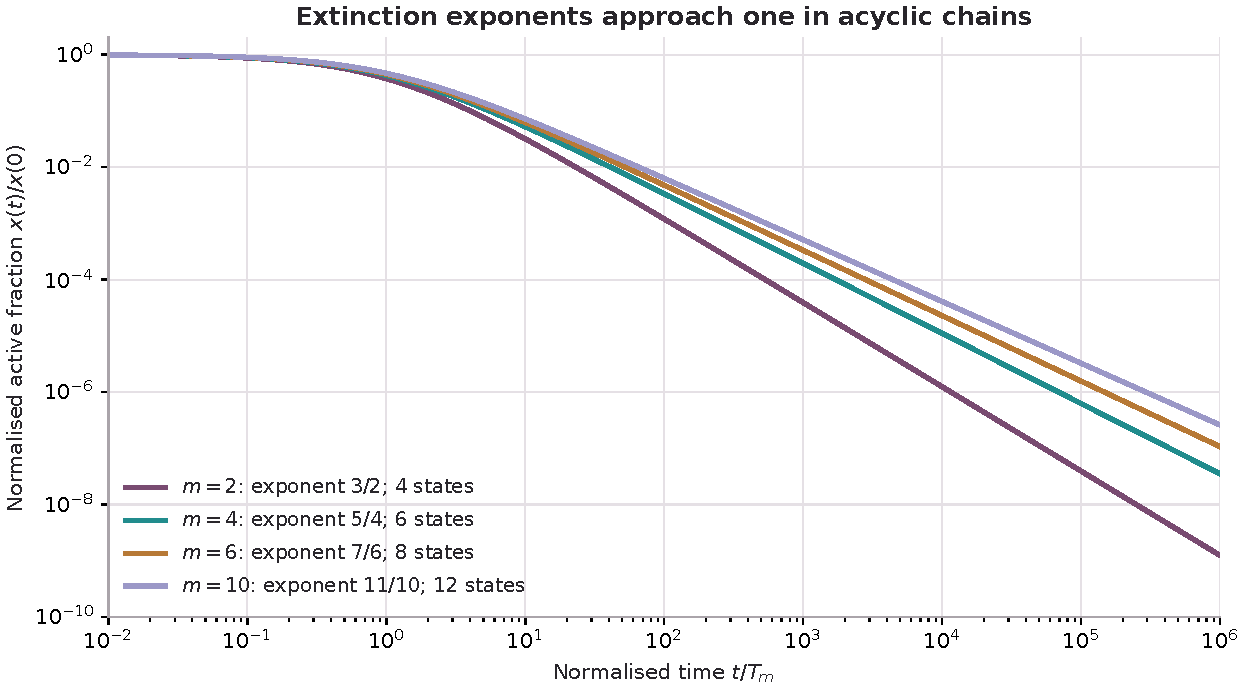
\includegraphics[width=.8\textwidth]{../figures/rate_hierarchy.pdf}
\caption{Hierarchy trajectories, activity normalised by its initial
value and time by $T_m$. Slopes approach $-1-1/m$. Illustration only.}
\label{fig:hierarchy}
\end{figure}}{}

\subsection{A sharp bound when one catalyst drives everything}

Many models in this paper (the base chain, SWIR, the hierarchy) have a
special property: every flux contains the active fraction $x$. Then the
whole system has the global form
\begin{equation}
\dot y=x\,Hy,\qquad H\ \text{constant},
\label{eq:linear_exposure}
\end{equation}
as an identity of polynomial vector fields on the simplex, and the
exposure clock linearises it globally: $y(t)=e^{Hu(t)}y(0)$ and
$x(t)=\Phi(u(t))$ with $\Phi(u)=e_x^{\mathsf T}e^{Hu}y(0)$. Since
$\one^{\mathsf T}\dot y=0$ identically, $\one^{\mathsf T}H=0$.

\begin{proposition}[Sharp dimension and parity bound]
\label{prop:dimension}
Let~\eqref{eq:linear_exposure} be an $N$-state model satisfying
(G1)--(G2) with interior data and $x\to0$, and let $U=\int_0^\infty x<\infty$.
Then $\Phi$ has a zero at $U$ of finite order $k$ with
$1\le k\le M_N=2\lfloor N/2\rfloor-1$. If $\Phi(U-v)=a_kv^k+O(v^{k+1})$
with $a_k>0$, then $k=1$ gives $x\sim Ce^{-a_1t}$ for some $C>0$, and
$k\ge2$ gives
\begin{equation}
x(t)\sim a_k^{-1/(k-1)}(k-1)^{-k/(k-1)}\,t^{-k/(k-1)}.
\label{eq:multiplicitytail}
\end{equation}
For $N\ge4$ the algebraic exponent is at least $M_N/(M_N-1)$. This is
attained in every $N\ge4$ with positive rational data and two acyclic
graphs; for odd $N$ by duplicating the terminal compartment.
\end{proposition}
\begin{proof}
\emph{Step 1 (order at most $N-1$).} By Lemma~\ref{lem:integrability},
$U<\infty$; $\Phi>0$ on $[0,U)$ and $\Phi(U)=0$. By Cayley--Hamilton,
$\Phi$ solves the order-$N$ linear constant-coefficient equation given by
the characteristic polynomial of $H$. If $\Phi$ and its first $N-1$
derivatives vanished at $U$, then $\Phi\equiv0$, contradicting
$\Phi(0)=x_0>0$. So $1\le k\le N-1$, and $a_k>0$ by positivity to the
left of $U$.

\emph{Step 2 (structure).} Every nonzero flux contains $x$: with the
topological weight $L=\sum_iiy_i$, the identity~\eqref{eq:linear_exposure}
gives $\dot L=0$ on the face $\{x=0\}$, while the contact form gives
$\dot L=\sum(j-i)\varphi_{ijk}$ with positive weights; at a point of the
face with all other fractions positive, a flux without the factor $x$
would make $\dot L>0$. Write the other $n=N-1$ coordinates as $z$, so
$\dd z/\dd u=Bz+b\Phi(u)$ with $B$ Metzler and $b\ge0$ (a negative entry
can only be a donor's own outflow). The transition graph has a sink
$j\ne X$ (a sink $X$ could not vanish), and $B_{jj}\ge0$; hence
$\sigma_B=s(B)\ge0$.

\emph{Step 3 (parity).} Suppose $k=n$. Let $z^*=z(U)$,
$g(v)=\one^{\mathsf T}e^{Bv}z^*$ and $\chi(\lambda)=\det(\lambda I-B)$.
Conservation and $\Phi(U)=0$ give $g(0)=1$. Since
$\Phi^{(j)}(U)=0$ for $j<n$, induction on $j$ in
$z^{(j+1)}=Bz^{(j)}+b\Phi^{(j)}$ gives $z^{(j)}(U)=B^jz^*$ for $j\le n$.
Differentiating conservation then yields $g^{(j)}(0)=0$ for $1\le j<n$
and $\Phi^{(n)}(U)=-g^{(n)}(0)$; Cayley--Hamilton for $B$ gives
\begin{equation}
\Phi^{(n)}(U)=\chi(0)\ne0 .
\label{eq:parityjet}
\end{equation}
The spectral abscissa of a Metzler matrix is an eigenvalue, so
$\chi(0)\ne0$ and $\sigma_B\ge0$ give $\sigma_B>0$. As $e^{Bv}\ge0$ and
$z^*\ge0$ has mass one, $g>0$, and its Laplace transform converges and is
positive for real $\lambda>\sigma_B$. Using $\chi(D)g=0$ and the initial
derivatives,
\begin{equation}
0<\int_0^\infty e^{-\lambda v}g(v)\dd v=\frac{\chi(\lambda)-\chi(0)}{\lambda\chi(\lambda)},
\qquad\lambda>\sigma_B .
\label{eq:paritylaplace}
\end{equation}
As $\lambda\downarrow\sigma_B$, $\chi(\lambda)\downarrow0$ through
positive values, so the right side has the sign of $-\chi(0)$: hence
$\chi(0)<0$. Positivity of $\Phi$ before $U$ requires
$(-1)^n\Phi^{(n)}(U)>0$, so with~\eqref{eq:parityjet} $n$ is odd. Thus
$k=N-1$ is impossible for odd $N$, and $k\le M_N$.

\emph{Step 4 (rates and sharpness).} With $v=U-u$,
$\dot v=-a_kv^k(1+O(v))$; for $k=1$ the logarithmic remainder is
integrable, and for $k\ge2$, $\dd(v^{1-k})/\dd t\to(k-1)a_k$,
giving~\eqref{eq:multiplicitytail}. For even $N=m+2$ the hierarchy has
$\Phi(u)=\varrho(e^{U-u}-1)^{m+1}e^{-(U-u)}$, of order $m+1=M_N$. For odd
$N\ge5$, take the hierarchy with $N-1$ states and split $R$ into $R_1,R_2$
with $r_1=r_2=r/2$, replacing $X\to R$ by the four moves
$X\to R_i$ catalysed by $R_j$ with flux $\tfrac12xr_j$. Then
$\dot r_i=\tfrac12(r_1+r_2)x$, the active trajectory is unchanged, the
graphs stay acyclic, and the order is $N-2=M_N$.
\end{proof}
The Cayley--Hamilton bound in Step 1 is standard; the parity step is
what uses positivity, acyclicity and conservation. The odd-dimensional
sharpness is obtained by duplication and adds no new dynamics.
The proposition concerns only the class~\eqref{eq:linear_exposure}.

\begin{corollary}[Slowest tail at $N=4$ with one vanishing state]
\label{cor:fourslowest}
Let $N=4$, (G1)--(G2) hold, the data be interior, and exactly one
compartment vanish. Then that compartment is $O(t^{-3/2})$, and either
it decays exponentially or like $t^{-2}$ or $t^{-3/2}$. The bound is
attained by Theorem~\ref{thm:base}.
\end{corollary}
\begin{proof}
If only $X$ vanishes, \eqref{eq:fluxzero} forces every nonzero flux to
contain $x$, so the model has the form~\eqref{eq:linear_exposure}.
Proposition~\ref{prop:dimension} gives $k\le M_4=3$.
\end{proof}

\subsection{The slowest tail with four compartments}
\label{sec:fourstate}
\emph{Goal: show that at $N=4$ nothing slower than $t^{-3/2}$ is
possible, whatever the topology and however many compartments vanish.}

Fix $N=4$, (G1)--(G2) and interior data, and order compartments
topologically, so compartment $1$ has no inflow and compartment $4$ no
outflow; $y_4$ never decreases and persists, so $\Vs\subset\{1,2,3\}$.
By~\eqref{eq:fluxzero} every active flux contains a vanishing factor, so
\begin{equation}
\dot v=J(p)v+\mathfrak N_1(v),\qquad \dot p=G(p)v+\mathfrak N_2(v),
\label{eq:split4}
\end{equation}
with $p=y_\Ps$, $v=y_\Vs$, matrices $J(p)$, $G(p)$ whose entries are linear
forms in $p$ ($J(p)$ Metzler, with $J(p^*)=J$ as in~\eqref{eq:Jentries}),
and quadratic forms $\mathfrak N_1,\mathfrak N_2$. The face $\{v=0\}$
consists of equilibria. When $|\Ps|=2$, say $\Ps=\{\ell,m\}$, write
$\pi=p_\ell/(p_\ell+p_m)$; then $J(p)=(1-|v|)J_{\rm f}(\pi)$ with $J_{\rm f}$
affine in $\pi$, where $|v|=\sum_{i\in\Vs}y_i$.

\begin{lemma}[Diagonal lower bound]
\label{lem:diag4}
For $i\in\Vs$ there is $C$ with $\dot y_i\ge y_i(J_{ii}(p)-C|v|)$, so
$J_{ii}(p(t))\ge0$ cannot hold for all large $t$.
\end{lemma}
\begin{proof}
Keep only the autocatalytic inflow $c_{aii}y_ay_i$ ($a\in\Ps$); outflow
with vanishing catalysts is at most $C|v|y_i$. If $J_{ii}(p)\ge0$ for
$t\ge T$ then $y_i(t)\ge y_i(T)\exp(-C\int_T^\infty|v|)>0$, since vanishing
coordinates are integrable (Lemma~\ref{lem:integrability}).
\end{proof}

\begin{lemma}[Desingularisation]
\label{lem:desing}
Let $\xi>0$ be $C^1$, $\xi\to0$, $\int_0^\infty\xi<\infty$, and $\pi(t)\to\pi_\infty$.
Let $\Psi$ be real-analytic near $\pi_\infty$ with $\Psi(\pi_\infty)=0$, $b$
Lipschitz there, and for large $t$
\[
\dot\xi=\xi(\Psi(\pi)+\rho_1),\qquad \dot\pi=\xi(b(\pi)+\rho_2),\qquad
|\rho_1|+|\rho_2|\le C\xi .
\]
Then $\Psi\not\equiv0$, $b_\infty=b(\pi_\infty)\ne0$, and with $m$ the order
of the zero of $\Psi$ and $k=m+1$,
$C_\infty=-\Psi^{(m)}(\pi_\infty)(-b_\infty)^m/(k\,m!)>0$ and
$\xi(t)\sim C_\infty((k-1)C_\infty t)^{-k/(k-1)}$.
\end{lemma}
\begin{proof}
In exposure time $u=\int\xi$ (finite total $U$),
$\dd\xi/\dd u=\Psi(\pi)+\rho_1$, $\dd\pi/\dd u=b(\pi)+\rho_2$. If
$b_\infty=0$, then $X=(\pi-\pi_\infty,\xi)$ obeys $|\dd X/\dd u|\le C|X|$,
so $|X|$ stays bounded below on $[u_1,U)$, contradicting $X\to0$. If
$\Psi\equiv0$, then $|\dd\xi/\dd u|\le C\xi$ and $\xi$ is bounded below
likewise. So $b_\infty\ne0$ and $m<\infty$. Then
$\pi-\pi_\infty=-(b_\infty+o(1))(U-u)$ and
$\Psi(\pi(u))=(L+o(1))(U-u)^m$ with
$L=\Psi^{(m)}(\pi_\infty)(-b_\infty)^m/m!$. With $M(u)=\sup_{[u,U)}\xi$,
$\xi(u)=\int_u^U(-\Psi-\rho_1)$ gives $M\le C_1(U-u)^{m+1}+C(U-u)M$, hence
$M=O((U-u)^{m+1})$, $\int_u^U|\rho_1|=O((U-u)^{m+2})$ and
$\xi=(-L/k+o(1))(U-u)^k$, so $C_\infty=-L/k>0$. Finally $\tau=U-u$ obeys
$\dot\tau=-(C_\infty+o(1))\tau^k$, which gives the stated law.
\end{proof}

\begin{theorem}[Slowest tail at $N=4$]
\label{thm:four}
With $N=4$, (G1)--(G2) and interior data, every vanishing coordinate either
decays exponentially or satisfies $y_i\sim C_it^{-2}$ or $y_i\sim C_it^{-3/2}$
with $C_i>0$. In particular every vanishing coordinate is $O(t^{-3/2})$,
and the exponent $3/2$ is attained (Theorem~\ref{thm:base}).
\end{theorem}
\begin{proof}
\emph{$|\Vs|=1$:} Corollary~\ref{cor:fourslowest}.

\emph{$\Vs=\{1,2,3\}$:} $\Ps=\{4\}$ and compartment $4$ donates nothing,
so the only off-diagonal entries of $J$ come from a vanishing donor $j$
with catalyst $4$, which requires $j<i$. Thus $J$ is lower triangular with
diagonal $-h_i^*<0$ (Lemma~\ref{lem:integrability}), and
Theorem~\ref{thm:spectral} gives exponential decay.

\emph{$\Vs=\{1,i\}$, $i\in\{2,3\}$:} $y_1$ has no inflow and hazard
$h_1\to h_1^*>0$, so it decays exponentially; row $1$ of $J$ is
$(-h_1^*,0)$, so if $J_{ii}<0$ all decay is exponential. Let $J_{ii}=0$.
Every inflow into $i$ not proportional to $y_i$ contains $y_1$, so
$\dot y_i=y_i(J_{ii}(p)+O(|v|))+y_1R$ with $R\ge0$ bounded. With
$4\omega=h_1^*$, eventually $y_1\le Ce^{-3\omega t}$, while
$\dot y_i/y_i\ge J_{ii}(p)+O(|v|)\to0$ gives $y_i\ge ce^{-\omega t}$; hence
$y_1/y_i=O(y_i^2)$. So $\xi=y_i$, $\Psi(\pi)=J_{ii}(p_{\rm f}(\pi))$ and the
face coordinate $\pi$ satisfy Lemma~\ref{lem:desing}. $\Psi$ is affine
and not identically zero, so $m=1$: decay $t^{-2}$.

\emph{$\Vs=\{2,3\}$:} $\Ps=\{1,4\}$ and $\pi=y_1/(y_1+y_4)$ is
nonincreasing because $\dot y_1\le0\le\dot y_4$, so $\pi\downarrow\pi_\infty$.
The affine functions $g_i(\pi)=J_{ii}(p_{\rm f}(\pi))$ satisfy
$g_i(0)=-h_i(e_4)\le0$, since compartment $4$ donates nothing. If
$g_i(\pi_\infty)\ge0$, then $g_i$ is nondecreasing, so $g_i(\pi(t))\ge0$ for
all $t$, contradicting Lemma~\ref{lem:diag4}. Hence $J_{22},J_{33}<0$. If
$J$ is reducible, or irreducible with $s(J)<0$, decay is exponential. It
remains to treat irreducible $J$ with $\det J=0$. Near $p^*$, the Perron
root $\lambda(p)$ of $J(p)$ is simple and analytic, with positive analytic
left and right eigenvectors $\psi(p)$, $\varsigma(p)$ ($\psi\cdot\varsigma=1$);
the other eigenvalue tends to $\operatorname{tr}J<0$. Put
$\xi=\psi(p)\cdot v\ge c|v|$. By~\eqref{eq:split4},
$\dot\xi=\xi(\lambda_{\rm f}(\pi)+\rho_1)$ with $|\rho_1|\le C\xi$. The
direction $q=v/\xi$ satisfies $\psi(p)\cdot q=1$ and, by~\eqref{eq:split4}
with $\dot p=O(\xi)$, $\dot q=(J(p)-\lambda(p))q+O(\xi)$. Let $\lambda_2(p)$ be
the other eigenvalue, with right eigenvector $\mathbf r_2(p)$ and left
vector $\omega_2(p)$ normalised by $\omega_2\cdot\mathbf r_2=1$,
$\omega_2\cdot\varsigma=0$, and write $q=\varsigma(p)+e_\perp\mathbf r_2(p)$.
Then $\dot e_\perp=(\lambda_2-\lambda)e_\perp+O(\xi)$. Since
$\lambda_2-\lambda\to\operatorname{tr}J<0$, there are $c>0$ and $T$ with
$\lambda_2-\lambda\le-2c$ and $|\dot\xi/\xi|\le c$ on $[T,\infty)$. Then
$\xi(\sigma)\le\xi(t)e^{c(t-\sigma)}$ for $T\le\sigma\le t$, and variation of
constants gives
$|e_\perp(t)|\le e^{-2c(t-T)}|e_\perp(T)|+C\int_T^te^{-2c(t-\sigma)}\xi(\sigma)\dd\sigma
\le C'\xi(t)$, using also $e^{-2c(t-T)}\le e^{-c(t-T)}\le\xi(t)/\xi(T)$.
Hence $|v/\xi-\varsigma(p)|\le C\xi$.
Hence $\dot\pi=\xi(b(\pi)+\rho_2)$ with $b$ analytic and $|\rho_2|\le C\xi$.
Lemma~\ref{lem:desing} applies to $\Psi=\lambda_{\rm f}$. Near $\pi_\infty$,
$\det J_{\rm f}=\lambda_{\rm f}\cdot(\text{a negative function})$, so $m$ is the
order of the zero of $\det J_{\rm f}$, a nonzero polynomial of degree at
most two. Thus $k\in\{2,3\}$, and both coordinates follow the same law
because $v\sim\xi\,\varsigma(p^*)$ with $\varsigma(p^*)>0$.
\end{proof}

\begin{remark}[Examples with two vanishing compartments; numerical]
\label{rem:e4}
The model $\dot y_1=-By_1y_3$, $\dot y_2=By_1y_3-y_2y_4-y_2y_1$,
$\dot y_3=y_2y_4-y_3y_4-y_3y_1$, $\dot y_4=y_2y_1+y_3y_4+y_3y_1$ satisfies
(G1), and (G2) whenever $\Vs=\{2,3\}$ (the only dependency cycle is
$1\to3\to1$). On the face,
$J_{\rm f}(\pi)=\bigl(\begin{smallmatrix}-1&B\pi\\1-\pi&-1\end{smallmatrix}\bigr)$
and $\lambda_{\rm f}=-1+\sqrt{B\pi(1-\pi)}$. For $B=4$ the root is double at
$\pi=1/2$, with predicted $t^{3/2}(y_2+2y_3)\to\sqrt3/2$; for $B=9/2$ it is
simple at $\pi=2/3$, with predicted $t^2(y_2+3y_3)\to16/3$. Near-critical
interior data found by bisection give $0.806,0.844,0.859,0.870$ and
$5.07,5.25,5.31,5.33$ at $t=10^4,10^{4.5},10^5,10^{5.5}$ (package script
\texttt{check\_four\_state.py}). Existence of interior data landing
exactly on these zeros is supported numerically but not proved, and
whether a $t^{-2}$ tail occurs when $\Vs=\{1,i\}$ is open. The argument
uses that the face of equilibria is at most a curve, which fails for
$N\ge5$.
\end{remark}


\section{The four-state chain: complete analysis}
\label{sec:chain}

\emph{Goal: for the simplest counterexample topology, describe every
trajectory, show that algebraic extinction is non-generic, quantify how
quickly exponential decay returns, and show that the slow tails never
follow an outbreak.}

\subsection{Classification}
Consider the chain with arbitrary rates,
\begin{equation}
\dot s=-\alpha sx,\qquad \dot w=\alpha sx-\beta wx,\qquad
\dot x=(\beta w-\gamma r)x,\qquad \dot r=\gamma rx,
\label{eq:generalchain}
\end{equation}
$\alpha,\beta,\gamma>0$, interior data. In exposure time
$s=s_0e^{-\alpha u}$, $r=r_0e^{\gamma u}$,
$w=w_0e^{-\beta u}+\frac{\alpha s_0}{\beta-\alpha}(e^{-\alpha u}-e^{-\beta u})$
for $\alpha\ne\beta$ and $w=e^{-\alpha u}(w_0+\alpha s_0u)$ for
$\alpha=\beta$, and $\Phi=1-s-w-r$, with
\begin{equation}
\Phi'=\beta w-\gamma r,\quad
\Phi''=\alpha\beta s-\beta^2w-\gamma^2r,\quad
\Phi'''=-\alpha\beta(\alpha+\beta)s+\beta^3w-\gamma^3r .
\label{eq:profilederivatives}
\end{equation}

\begin{theorem}[All rates and all interior data]
\label{thm:classification}
$\Phi$ has a first positive zero $U$, $u(t)\uparrow U$, $x\to0$, and
$s,w,r$ have positive limits. Exactly one of the following holds.
\begin{enumerate}[label=(\roman*)]
\item $\omega_*=\gamma r^*-\beta w^*>0$: $x(t)\sim Ce^{-\omega_*t}$, $C>0$.
\item $\beta w^*=\gamma r^*$ and $\kappa=\alpha\beta s^*-\gamma(\beta+\gamma)r^*>0$:
$x(t)\sim2/(\kappa t^2)$.
\item $\beta w^*=\gamma r^*$ and $\kappa=0$: the endpoint is
\begin{equation}
s^*=\frac\gamma{\alpha+\gamma},\quad
w^*=\frac{\alpha\gamma}{(\alpha+\gamma)(\beta+\gamma)},\quad
r^*=\frac{\alpha\beta}{(\alpha+\gamma)(\beta+\gamma)},
\label{eq:tripleendpoint}
\end{equation}
and $x(t)\sim\frac{\sqrt3}{2\sqrt{\alpha\beta\gamma}}\,t^{-3/2}$.
\end{enumerate}
No higher order occurs, and for every rate triple all three cases
occur for suitable interior data.
\end{theorem}
\begin{proof}
$s,w,r>0$ for finite $u$ and $\Phi(0)=x_0>0$; eventually $r_0e^{\gamma u}>1$,
so $\Phi$ has a first zero $U$. The solution of $\dot u=\Phi(u)$
increases to $U$ without reaching it. Since $\Phi>0$ on $[0,U)$,
$\Phi'(U)\le0$. Case (i) is a simple zero
(Proposition~\ref{prop:dimension}, Step 4). If $\Phi'(U)=0$ then
$\Phi''(U)=\kappa\ge0$; $\kappa>0$ gives a double zero with
$a_2=\kappa/2$. If $\kappa=0$, solving the two conditions with
$s^*+w^*+r^*=1$ gives~\eqref{eq:tripleendpoint}, and substitution gives
$\Phi'''(U)=-\alpha\beta\gamma<0$, a triple zero with
$a_3=\alpha\beta\gamma/6$; this also excludes higher order.
\eqref{eq:multiplicitytail} gives the constants. For attainability, fix
an endpoint on the face $x=0$ with $\beta w^*<\gamma r^*$ (simple), with
$\beta w^*=\gamma r^*$ and
$0<r^*<\alpha\beta/((\alpha+\gamma)(\beta+\gamma))$ (double), or
\eqref{eq:tripleendpoint} (triple), and integrate the linear exposure
system backwards over a short interval; the sign of the leading Taylor
term (for the triple case, $\Phi'''(U)<0$) gives $\Phi>0$ just before
$U$, and continuity keeps the other fractions positive.
\end{proof}

For rates $(2,1,1)$ the profile is $\Phi=Q(q)/q$ with the cubic
\eqref{eq:cubic}, and the attained root is the largest root
$q_*\in(0,1)$; a multiple root below a simple root that is reached first
does not determine the tail. The double-zero data are exactly
\begin{equation}
s_0=\frac h{q_*^2},\quad w_0=\frac{3h+1}{2q_*}-\frac{2h}{q_*^2},\quad
r_0=\frac{q_*(1-h)}2,\qquad \frac13<h<1,\quad \frac{4h}{3h+1}<q_*<1,
\label{eq:doublefamily}
\end{equation}
with $Q=s_0(q-q_*)^2(q-q_\circ)$, $q_\circ=q_*(1-h)/(2h)$, endpoint
$(h,(1-h)/2,0,(1-h)/2)$ and $x\sim\frac2{3h-1}t^{-2}$. Indeed, write a
double root as $Q=s_0(q-q_*)^2(q-q_\circ)$. Then $q_\circ>0$ because
$r_0>0$; $q_\circ\ge1$ contradicts $Q(1)=x_0>0$; $q_\circ\in(q_*,1)$ would
be attained first; and $q_\circ=q_*$ is the triple case. Hence
$q_\circ<q_*$, which is $h>1/3$, and the remaining inequality is $w_0>0$.
Example~\eqref{eq:doubleexample} is $h=1/2$, $q_*=9/10$.

\subsection{Genericity}

\begin{theorem}[Algebraic extinction is non-generic]
\label{thm:generic}
Let~\eqref{eq:linear_exposure} be a model on the open simplex $\Omega$
(dimension $N-1$), and let $\Omega_0\subset\Omega$ be the set of data
for which $x$ is integrable (under (G1)--(G2), this is the set for which
$x$ vanishes). Let $\Omega_{\exp}\subset\Omega_0$ be the data for which
$x$ decays exponentially, and $E_k$ the data whose first zero has order
at least $k$. Then:
\begin{enumerate}[label=(\alph*)]
\item $\Omega_{\exp}$ is open in $\Omega$;
\item $E_2=\Omega_0\setminus\Omega_{\exp}$ has Lebesgue measure zero, so
$\Omega_{\exp}$ has full measure in $\Omega_0$; if $\Omega_0$ is open
(for example $\Omega_0=\Omega$), $\Omega_{\exp}$ is also dense in it;
\item $E_k$ is contained in the image under a smooth map of a manifold of
dimension $N-1-r_k$, where $r_k\le k-1$ is the rank of the affine
conditions $e_x^{\mathsf T}H^jy^*=0$ $(1\le j<k)$ on the face
$\{y_x=0,\ \one^{\mathsf T}y=1\}$, so its codimension is at least $r_k$;
the data of exact order $k$ form, locally, an immersed submanifold of
that dimension, and $E_k$ is the finite union of these strata.
\end{enumerate}
For the four-state chain~\eqref{eq:generalchain}, $\Omega_0=\Omega$,
and at fixed rates the $t^{-2}$ data form a surface (codimension one)
and the $t^{-3/2}$ data a curve (codimension two).
\end{theorem}
\begin{proof}
For $y_0\in\Omega$ write $\Phi_{y_0}(u)=e_x^{\mathsf T}e^{Hu}y_0$, which
is linear in $y_0$ and analytic in $u$. If $\Phi_{y_0}$ has a positive
zero, $u(t)$ increases to the first one, $U$, and $x$ is integrable;
conversely integrability gives $U<\infty$ and $\Phi_{y_0}(U)=0$. By
Proposition~\ref{prop:dimension} (Step 4, which uses only the form
\eqref{eq:linear_exposure}), $x$ decays exponentially iff the first zero
is simple.

(a) Let $U$ be a simple first zero of $\Phi_{y_0}$. Choose $\eta>0$ with
$\Phi_{y_0}'<0$ on $[U-\eta,U+\eta]$. For $y_1$ near $y_0$, $\Phi_{y_1}$
and $\Phi_{y_1}'$ are uniformly close to $\Phi_{y_0}$ and $\Phi_{y_0}'$
on $[0,U+\eta]$, so $\Phi_{y_1}>0$ on $[0,U-\eta]$, $\Phi_{y_1}'<0$ on
$[U-\eta,U+\eta]$, and $\Phi_{y_1}$ changes sign there. Its first zero
is therefore simple.

(b,c) Let $\Pi$ be the affine face $\{y_x=0,\one^{\mathsf T}y=1\}$
(dimension $N-2$) and $\Lambda(y^*,U)=e^{-HU}y^*$ on $\Pi\times(0,\infty)$;
since $\one^{\mathsf T}H=0$, $\Lambda$ maps into $\{\one^{\mathsf T}y=1\}$.
Every $y_0\in\Omega_0$ equals $\Lambda(y(U),U)$, and the pair is
determined by $y_0$. The first zero has order at least $k$ iff in
addition $\ell_j(y^*):=e_x^{\mathsf T}H^jy^*=\Phi^{(j)}(U)=0$ for
$1\le j<k$. If $\ell_1$ vanishes identically on $\Pi$ then, since $\Pi$
spans $\{y_x=0\}$, $\ell_1(y)=H_{xx}y_x$ and $\Phi'=H_{xx}\Phi$, so
$\Phi=x_0e^{H_{xx}u}$ never vanishes and $\Omega_0=\varnothing$.
Otherwise the conditions cut out an affine subspace $\Pi_k\subset\Pi$ of
dimension $N-2-r_k$ with $r_k\ge1$ for $k\ge2$, and
$E_k\subset\Lambda(\Pi_k\times(0,\infty))$. The differential of
$\Lambda$ at $(y^*,U)$ is $(\delta y,\delta U)\mapsto e^{-HU}(\delta y-Hy^*\delta U)$.
At a zero of exact order $k'\ge k$ the vector $Hy^*$ satisfies
$\ell_j(Hy^*)=\Phi^{(j+1)}(U)$, which vanishes for $j<k'-1$ and not for
$j=k'-1$, while $e_x^{\mathsf T}Hy^*=\Phi'(U)=0$; so $Hy^*$ is not
tangent to $\Pi_{k'}$, and $\Lambda$ restricted to $\Pi_{k'}\times(0,\infty)$
is an immersion at points of exact order $k'$ (at points of higher order
it need not be, which is why (c) is stated as a containment plus a
stratification by exact order $k'\in\{k,\dots,N-1\}$). A $C^1$ image of
a manifold of dimension $N-2$ in an $(N-1)$-dimensional space has
measure zero, which proves the first part of (b), and the same argument
with $\Pi_k$ proves (c). If $\Omega_0$ is open, the open set
$\Omega_{\exp}$ differs from it by a null set, which has empty
interior, so $\Omega_{\exp}$ is dense in $\Omega_0$.

For the chain, Theorem~\ref{thm:classification} gives $\Omega_0=\Omega$.
The double-zero condition $\ell_1=\beta w^*-\gamma r^*=0$ is one affine
condition on the two-dimensional face, and the triple endpoint
\eqref{eq:tripleendpoint} is a point, so $r_2=1$ and $r_3=2$. For rates
$(2,1,1)$ this is also visible in the explicit parameterisations: the
map $(h,q_*)\mapsto(s_0,w_0,r_0)$ in~\eqref{eq:doublefamily} has a
$2\times2$ minor $-(3h-1)/(2q_*^2)\ne0$, and the curve
\eqref{eq:triplefamily} has $\dd s_0/\dd q_*\ne0$ (exact check in the
package).
\end{proof}

Table~\ref{tab:codim} collects the resulting dictionary between the
order of the zero, the tail, the amount of tuning, and the response to
perturbation (Theorem~\ref{thm:slowing}).

\begin{table}[ht]
\centering\small
\begin{tabular}{lcccc}
\toprule
order $k$ of zero & tail of $x$ & codimension (chain) & relaxation rate & endpoint shift\\
\midrule
1 & $e^{-\omega t}$ & 0 (open set) & --- & $O(\varepsilon)$\\
2 (spinodal) & $t^{-2}$ & 1 & $\propto|\varepsilon|^{1/2}$ one side & $|\varepsilon|^{1/2}$ or jump\\
3 (tricritical) & $t^{-3/2}$ & 2 & $\propto|\varepsilon|^{2/3}$ & $\propto|\varepsilon|^{1/3}$\\
$k$ (class \eqref{eq:linear_exposure}) & $t^{-k/(k-1)}$ & $r_k\le k-1$ & $\propto|\varepsilon|^{(k-1)/k}$ & $|\varepsilon|^{1/k}$; jump if $k$ even\\
\bottomrule
\end{tabular}
\caption{Order of the zero, tail, tuning and response to a perturbation
of size $\varepsilon$.}
\label{tab:codim}
\end{table}

\subsection{How fast exponential decay returns}

\begin{theorem}[General-order slowing law]
\label{thm:slowing}
In the class~\eqref{eq:linear_exposure}, let $y_0$ have a first zero of
order $k\ge2$ at $U$, $\Phi(U-v)=a_kv^k+O(v^{k+1})$, $a_k>0$. Let
$\delta$ satisfy $\one^{\mathsf T}\delta=0$, put
$\Gamma(u)=e_x^{\mathsf T}e^{Hu}\delta$ and assume $g=\Gamma(U)\ne0$.
For small $\varepsilon\ne0$ consider the data $y_0+\varepsilon\delta$.
\begin{enumerate}[label=(\alph*)]
\item If $k$ is odd, or $k$ is even and $\varepsilon g<0$, the first
zero $U_\varepsilon$ is simple,
$U_\varepsilon-U=\operatorname{sgn}(\varepsilon g)\,|\varepsilon g/a_k|^{1/k}(1+o(1))$,
and $x$ decays exponentially with rate
\begin{equation}
\omega_\varepsilon=k\,a_k^{1/k}\,|\varepsilon g|^{(k-1)/k}\,(1+o(1)).
\label{eq:slowinglaw}
\end{equation}
\item If $k$ is even and $\varepsilon g>0$, there is $\eta>0$,
independent of $\varepsilon$, with $\Phi_\varepsilon>0$ on $[0,U+\eta]$:
the endpoint jumps by at least $\eta$ in exposure.
\end{enumerate}
In case (a) the endpoint moves by
$y^*_\varepsilon-y^*=Hy^*\,\Delta U+O\bigl((\Delta U)^2+|\varepsilon|\bigr)$,
$\Delta U=U_\varepsilon-U$, with $Hy^*\ne0$: a shift of order
$|\varepsilon|^{1/k}$.
\end{theorem}
\begin{proof}
$\Phi_\varepsilon=\Phi+\varepsilon\Gamma$ by linearity. Fix a small
$\eta>0$ such that $\Phi'<0$ on $[U-\eta,U)$, $\Phi$ has no zero in
$(U,U+\eta]$ when $k$ is even, and $|\Phi(U-v)-a_kv^k|\le a_k|v|^k/4$
for $|v|\le\eta$. On $[0,U-\eta]$, $\Phi\ge c>0$, so
$\Phi_\varepsilon>0$ there for small $\varepsilon$. Substitute
$v=|\varepsilon|^{1/k}\tau$. Uniformly for $\tau$ in compact sets,
$|\varepsilon|^{-1}\Phi_\varepsilon(U-v)=a_k\tau^k+\operatorname{sgn}(\varepsilon)g+O(|\varepsilon|^{1/k})$.
In case (a) the limit polynomial has exactly one real root
$\tau_0=-\operatorname{sgn}(\varepsilon g)|g/a_k|^{1/k}$ on the relevant
side, and it is simple. When $k$ is even and $\varepsilon g<0$ the
other root $-\tau_0$ lies beyond $\tau_0$ in $u$. The implicit function
theorem gives a simple zero $\tau_\varepsilon\to\tau_0$, and positivity
of $a_k\tau^k+\operatorname{sgn}(\varepsilon)g$ before $\tau_0$, together with the
bound on $[U-\eta,U-|\varepsilon|^{1/k}T]$ for large $T$, shows that it
is the first zero. Then
$-\Phi_\varepsilon'(U_\varepsilon)=ka_kv_\varepsilon^{k-1}(1+o(1))+O(\varepsilon)$
with $|v_\varepsilon|\sim|\varepsilon g/a_k|^{1/k}$, and
$\varepsilon=o(|\varepsilon|^{(k-1)/k})$, which
gives~\eqref{eq:slowinglaw}; the rate of $x$ is $-\Phi_\varepsilon'$ at
its simple first zero (Proposition~\ref{prop:dimension}, Step 4). In
case (b), $\Phi_\varepsilon\ge\Phi+\varepsilon\min\Gamma>0$ on
$[U-\eta,U+\eta]$ once $\varepsilon$ is small, since $\Phi\ge0$ there
and $\Gamma$ has the sign of $g$ near $U$. Finally
$y^*_\varepsilon=e^{HU_\varepsilon}(y_0+\varepsilon\delta)
=e^{H\Delta U}y^*+\varepsilon e^{HU_\varepsilon}\delta
=y^*+Hy^*\Delta U+O((\Delta U)^2+|\varepsilon|)$, and $Hy^*=0$
would make $y^*$ an equilibrium of the exposure flow reached at finite
$U$, forcing $\Phi\equiv0$.
\end{proof}

For the base chain with $x_0\mapsto x_0+\varepsilon$,
$r_0\mapsto r_0-\varepsilon$ we have $a_3=1/3$, $g=5/4$, and
\eqref{eq:slowinglaw} reproduces the exact rate
$3(25/48)^{1/3}|\varepsilon|^{2/3}$, which here holds for every
admissible $\varepsilon\ne0$ because $Q_\varepsilon=\frac{25}{48}(q-\frac45)^3+\varepsilon$.
For the double-zero example~\eqref{eq:doubleexample} with the same
perturbation, $\varepsilon<0$ gives a rate
$\approx2\cdot\frac12|\tfrac{10}9\varepsilon|^{1/2}$, while $\varepsilon>0$
moves the attained root from $9/10$ to $9/20$: the final stifler
fraction jumps from $1/4$ to $1/2$ and the final unaware fraction from
$1/2$ to $1/8$. This discontinuity of the final state across the
codimension-one double-zero surface is a spinodal; the triple-zero curve
is where the jump closes, a tricritical point in the sense used for
generalised epidemics~\cite{Janssen,Bizhani,ChoiLeeKahng} and for the
discontinuous transitions of complex contagion~\cite{DoddsWatts,ChenCoinfection}.
The package checks~\eqref{eq:slowinglaw} at high precision for these
two examples and for the order-five zero of the $m=4$ hierarchy.
The relaxation time $\omega_\varepsilon^{-1}\propto|\varepsilon|^{-(k-1)/k}$
is a critical-slowing-down law of the kind used as an early-warning
indicator of elimination~\cite{ORegan}.

\IfFileExists{../figures/critical_dynamics.pdf}{%
\begin{figure}[ht]
\centering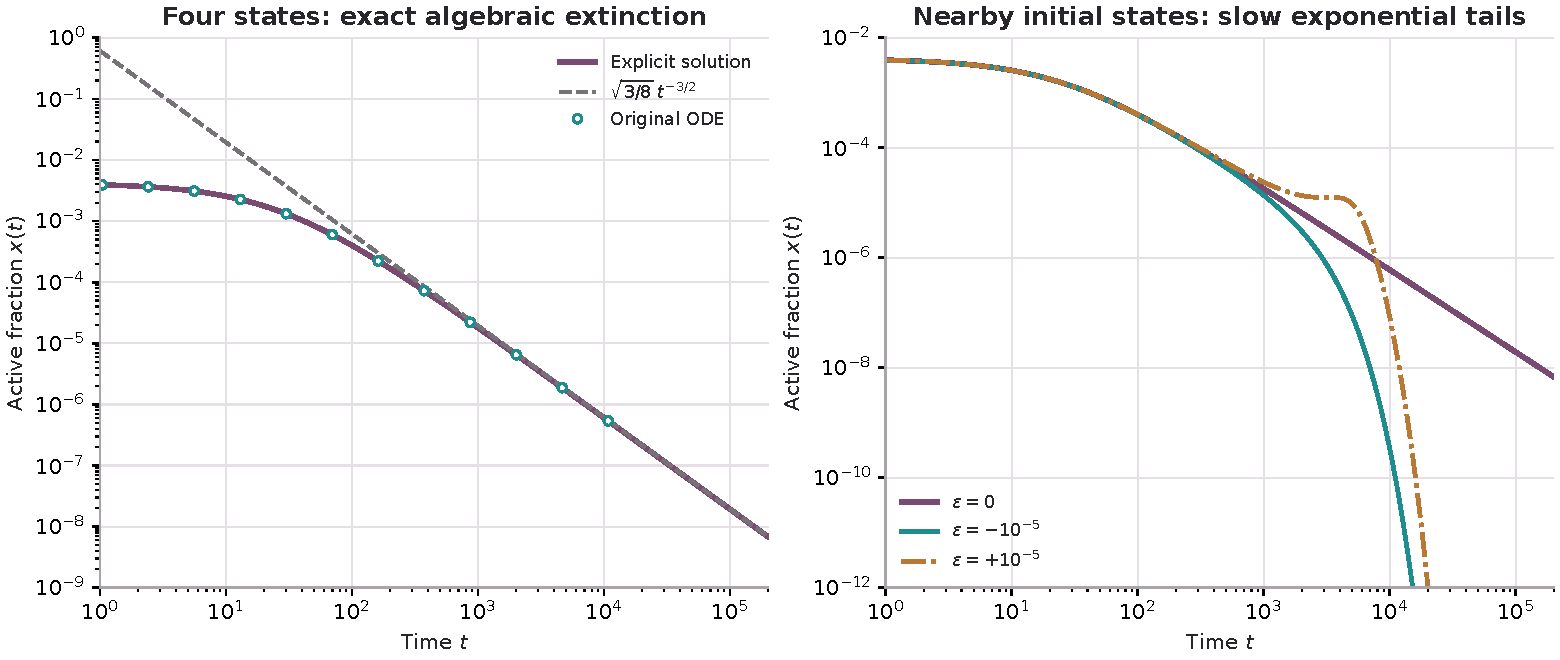
\includegraphics[width=\textwidth]{../figures/critical_dynamics.pdf}
\caption{Left: the explicit trajectory of Theorem~\ref{thm:base}, a
numerical integration of~\eqref{eq:base}, and the asymptote
$\sqrt{3/8}\,t^{-3/2}$. Right: perturbations $\varepsilon=\pm10^{-5}$
of $(x_0,r_0)$; both decay exponentially at the rate of
Theorem~\ref{thm:slowing}. Illustration only.}
\label{fig:critical}
\end{figure}}{}

\subsection{No outbreak precedes a slow tail}

\begin{lemma}[Zeros of exponential polynomials]
\label{lem:zeros}
Let $f(u)=\sum_{j=1}^np_j(u)e^{\lambda_ju}$ with distinct real $\lambda_j$
and nonzero real polynomials $p_j$ of degrees $d_j$. Then $f$ has at most
$D-1$ real zeros counted with multiplicity, where $D=\sum_j(d_j+1)$.
\end{lemma}
\begin{proof}
Induction on $D$; $D=1$ is clear. Multiply by $e^{-\lambda_nu}$ and
differentiate $d_n+1$ times. This removes the $n$-th term and leaves an
exponential polynomial with the other $\lambda_j-\lambda_n\ne0$ and the
same degrees, which has at most $D-d_n-2$ zeros by induction. Rolle's
theorem, counted with multiplicity, gives at most
$(D-d_n-2)+(d_n+1)=D-1$ zeros for $f$. (This is a classical
generalisation of Descartes' rule; see~\cite{PolyaSzego}.)
\end{proof}

\begin{proposition}[Monotone fade-out]
\label{prop:nopeak}
In the following cases $x(t)$ is strictly decreasing on $[0,\infty)$, so
the largest activity is the initial one:
\begin{enumerate}[label=(\alph*)]
\item the chain~\eqref{eq:generalchain}, any rates, whenever the first
zero is double or triple;
\item SWIR~\eqref{eq:swir}, any $\nu,\eta>0$, whenever the first zero is
double or triple;
\item the hierarchy~\eqref{eq:familytrajectory}, every even $m$.
\end{enumerate}
\end{proposition}
\begin{proof}
Since $\dot x=\Phi'(u)x$, it suffices that $\Phi'<0$ on $[0,U)$.
(a) $\Phi'=\beta w-\gamma r$ is an exponential polynomial with $D=3$
(exponents $-\alpha,-\beta,\gamma$; or $-\alpha$ with degree one and
$\gamma$ when $\alpha=\beta$), so it has at most two real zeros, and
$\Phi'(u)\to-\infty$ as $u\to\infty$. At a triple zero, $U$ is a double
zero of $\Phi'$, so $\Phi'$ has no other zero, and it is negative near
$U$. At a double zero, $\Phi'(U)=0<\Phi''(U)$, so $\Phi'$ crosses
upwards at $U$; since it ends negative, it has a second zero after $U$,
hence none before, and it is negative just before $U$. In both cases
$\Phi'<0$ on $(-\infty,U)$.
(b) $\Phi'=\eta w-1$ has exponents $-\nu,-\eta,0$ (or degree one at
$-\eta$ if $\nu=\eta$), so $D=3$, and $\Phi'\to-1$; the argument of (a)
applies.
(c) From~\eqref{eq:familytrajectory},
$w_1=\varrho\zeta\sum_{\ell=0}^{m-1}(\ell+1)(-\vartheta)^\ell
=\varrho(1-(m+1)\vartheta^m-m\vartheta^{m+1})/\zeta$, so
$w_1-r=-\varrho\vartheta^m(m+1+m\vartheta)/\zeta<0$.
\end{proof}
For the base trajectory this is explicit:
$w-r=-(\zeta-1)^2(2\zeta+1)/(3\zeta)<0$. So in these families the slow
tail is a slow fade-out from a subcritical start
($R_{\mathrm{eff}}<1$ throughout), not the end of an epidemic wave.
Whether some model in the class has an algebraic tail after a genuine
peak is open (Section~\ref{sec:discussion}).

\section{What replaces the conjecture}
\label{sec:spectral}

\emph{Goal: identify exactly what goes wrong, and give conditions,
checkable from the coefficient supports or the rates, under which the conjectured
conclusion is true.}

Assume (G1), let $y^*$ be the limit, $\Vs$ and $\Ps$ the vanishing and
persistent sets, $v=y_\Vs$, and assume $\Vs\ne\varnothing$. Let $J$ be
the Jacobian of the vanishing right-hand sides with respect to $v$ at
$(y_\Ps^*,0)$. Collecting the terms of~\eqref{eq:model} that are linear
in $v$ at the limit, and using~\eqref{eq:fluxzero}, for $i\ne j$ in $\Vs$
\begin{equation}
J_{ii}=\sum_{a\in\Ps}c_{aii}y_a^*-\sum_{k\in\Ps}h_{ik}y_k^*,\qquad
J_{ij}=\sum_{k\in\Ps}c_{jik}y_k^*+\sum_{a\in\Ps}c_{aij}y_a^*,\qquad
h_{ik}=\sum_{b\ne i}c_{ibk}.
\label{eq:Jentries}
\end{equation}
The first sum in $J_{ii}$ is \emph{autocatalytic inflow}: a persistent
donor moving into $i$ on contact with $i$ itself. $J$ is Metzler.

\begin{theorem}[Logarithmic decay rate from the limiting block]
\label{thm:spectral}
Under (G1), with interior data,
\begin{equation}
\lim_{t\to\infty}\frac1t\log\norm{v(t)}_1=s(J)\le0 .
\label{eq:lograte}
\end{equation}
Every vanishing coordinate has an exponential bound iff $s(J)<0$, and
then $\norm{y(t)-y^*}_1\le C_\omega e^{-\omega t}$ for every
$0<\omega<-s(J)$.
\end{theorem}
\begin{proof}
\emph{Step 1.} Every nonzero flux has a factor in $\Vs$
by~\eqref{eq:fluxzero}. Write each inflow into a vanishing coordinate as
a nonnegative coefficient times one vanishing factor (if both factors
vanish, choose one; if the catalyst is the destination itself, the
coefficient goes on the diagonal), and put each outflow on the donor's
diagonal. This gives $\dot v=M(t)v$ with $M(t)$ Metzler, since only
diagonal entries can be negative, and $M(t)\to J$; terms with two
vanishing factors contribute coefficients tending to zero.

\emph{Step 2 (upper bound).} For $\mu>s(J)$,
$\theta=(\mu I-J^{\mathsf T})^{-1}\one=\int_0^\infty e^{(J^{\mathsf T}-\mu)\sigma}\one\dd\sigma>0$
and $J^{\mathsf T}\theta=\mu\theta-\one$, so eventually
$M(t)^{\mathsf T}\theta\le\mu\theta$ and $W=\theta^{\mathsf T}v$ satisfies
$\dot W\le\mu W$. Hence $\limsup t^{-1}\log\norm v_1\le\mu$.

\emph{Step 3 (lower bound).} Choose an irreducible diagonal block $B$ of
the Frobenius form of $J$ with $s(B)=s(J)$, and a positive left
eigenvector $\psi$ (Perron--Frobenius~\cite{BermanPlemmons}). Off-block
terms are nonnegative, so $\dot v_B\ge M_B(t)v_B$, and $Z=\psi^{\mathsf T}v_B>0$
satisfies $\dot Z\ge(s(J)-\epsilon)Z$ eventually, for every $\epsilon>0$.
Since $v\to0$, $s(J)\le0$.

\emph{Step 4.} If $s(J)<0$, Step 2 with $\mu=-\omega$ gives
$\norm v_1\le Ce^{-\omega t}$; each flux has a vanishing factor, so
$\norm{\dot y_\Ps}_1\le C'\norm v_1$, and integrating from $t$ to
$\infty$ gives the bound on $y-y^*$. The converse follows
from~\eqref{eq:lograte}.
\end{proof}
The same result, with a different proof, is Theorem~7 and Corollary~8
of~\cite{EPprior}. It is an a~posteriori criterion: it needs the limit
$y^*$, uses only (G1), and when $s(J)=0$ it does not determine the slower rate. Step 2 is
the standard linear-functional test for Metzler
stability~\cite{Rantzer,FarinaRinaldi}. For the base chain and SWIR,
$J=[0]$ at the algebraic endpoints. The structure of~\eqref{eq:Jentries}
is what yields criteria without the limit.

\begin{definition}
The \emph{limiting influence graph} on $\Vs$ has an edge $j\to i$
($i\ne j$) when $c_{jik}>0$ for some $k\in\Ps$ or $c_{aij}>0$ for some
$a\in\Ps$. By~\eqref{eq:Jentries} and $y^*_\Ps>0$, this is exactly the
off-diagonal support of $J$.
\end{definition}

\begin{corollary}[A support-checkable repair]
\label{cor:graph}
Assume (G1)--(G2), interior data, an acyclic limiting influence graph,
and no autocatalytic inflow into vanishing states from persistent
donors ($c_{aii}=0$ for $a\in\Ps$, $i\in\Vs$). Then every vanishing state
decays exponentially, and $y\to y^*$ exponentially.
\end{corollary}
\begin{proof}
Acyclicity makes $J$ permutation-similar to a triangular matrix, so
$s(J)=\max_iJ_{ii}$. Without autocatalytic inflow,
$J_{ii}=-\sum_kh_{ik}y_k^*$. By Lemma~\ref{lem:integrability} $i$ has a
persistent dependency successor $k$, so $h_{ik}>0$ and $J_{ii}<0$. Apply
Theorem~\ref{thm:spectral}.
\end{proof}
The hypotheses of Corollary~\ref{cor:graph} are conditions on the
supports of the $c_{ijk}$ together with the labels $\Vs,\Ps$. They are
checkable from the graphs alone when the labels are: by the source's
Corollary~1~\cite[p.~22]{CCM}, this holds under (G1)--(G2) ``if the
persistent successor within each cycle of the dependency graph is
identifiable'' (for example, when the dependency graph is acyclic).
Without the acyclicity hypothesis, $s(J)=\max_iJ_{ii}$ can fail and the
triangular argument does not apply. The base chain violates exactly the
autocatalysis condition ($W\to X$ catalysed by $X$), and so does SWIR.
In the source's language, the dependency graph records the catalysts of
\emph{outflows} only; the counterexamples live in the catalysts of
\emph{inflows}. Whether this is the ``edge case'' mentioned
in~\cite[p.~32]{CCM} we cannot say.

\begin{corollary}[A rate-checkable repair]
\label{cor:rates}
Assume (G1)--(G2), interior data and an acyclic limiting influence graph.
If for every $i\in\Vs$
\begin{equation}
c_{kii}\le h_{ik}\ \text{for all }k\in\Ps,\ \text{with strict inequality for at least one }k\in\Ps,
\label{eq:dominance}
\end{equation}
then every vanishing state decays exponentially. No criterion that
depends only on the rates can decide, without the initial data, whether
an individual trajectory decays exponentially or algebraically: for the
chain~\eqref{eq:generalchain}, every rate triple admits both.
\end{corollary}
\begin{proof}
By~\eqref{eq:Jentries}, $J_{ii}=\sum_{k\in\Ps}(c_{kii}-h_{ik})y_k^*<0$
because all $y_k^*>0$; conclude as in Corollary~\ref{cor:graph}. The
second statement is the attainability part of
Theorem~\ref{thm:classification}.
\end{proof}
Condition~\eqref{eq:dominance} says that each persistent compartment
helps remove $i$ at least as strongly as it feeds $i$ in $i$'s presence.
In the base chain it fails for $k=W$ ($c_{WXX}=1>h_{XW}=0$). In SWIR with
recovery encoded as in the source, $c_{WXX}=\eta$ and $h_{XW}=1$, so
\eqref{eq:dominance} holds iff $\eta\le1$; then SWIR always fades out
exponentially, consistent with the triple-zero condition $w^*=1/\eta<1$.
For given rates \emph{and} data in the class~\eqref{eq:linear_exposure},
the test is the multiplicity of the first zero of the explicit function
$\Phi$; for rates $(2,1,1)$ it reduces to whether the discriminant of
$Q$ vanishes at the attained root, a finite exact computation.

\section{Finite populations (exploratory)}
\label{sec:finite}

\emph{Goal: indicate, without proof, what the deterministic tail means
for a population of finite size.}

The deterministic model is the large-population limit of a Markov
chain~\cite{Kurtz}. We simulated that chain for the base model, with
$N$ individuals, events $S\to W$, $W\to X$, $X\to R$ at rates $2SX/N$,
$WX/N$, $RX/N$ and initial counts in the exact
proportions~\eqref{eq:baseinitial}, by Gillespie's
method~\cite{Gillespie} with fixed seeds. Table~\ref{tab:gillespie}
compares the median time at which the last spreader stops with the
deterministic time $t_1(N)$ at which $Nx(t)=1$.

\begin{table}[ht]
\centering\small
\begin{tabular}{rrrrrr}
\toprule
$N$ & runs & median $T$ & 10--90\% of $T$ & $t_1(N)$ & median final $r$\\
\midrule
24{,}000 & 200 & 98 & 51--233 & 556 & 0.298\\
240{,}000 & 60 & 283 & 151--552 & 2{,}718 & 0.311\\
2{,}400{,}000 & 20 & 986 & 411--1{,}658 & 12{,}810 & 0.345\\
24{,}000{,}000 & 20 & 1{,}676 & 870--2{,}914 & 59{,}777 & 0.319\\
\bottomrule
\end{tabular}
\caption{Exploratory simulation of the base model (package script
\texttt{finite\_population\_gillespie.py}).}
\label{tab:gillespie}
\end{table}

The median extinction time fits $1.48\,N^{0.42}$ (bootstrap 95\%
interval for the exponent $[0.38,0.46]$), whereas $t_1(N)$ grows like
$N^{2/3}$. A branching-process heuristic predicts $N^{2/5}$: a near-critical
population of $n$ spreaders dies out on a time scale of order $n$, and
the deterministic count $Nx(t)\sim N t^{-3/2}$ falls to order $t$ once
$t\gtrsim N^{2/5}$.
At these sizes the deterministic tail overestimates the time to
extinction by a factor of 6 to 36. Fluctuations of order $N^{-1/2}$ in
the realised fractions act like the perturbation $\varepsilon$ of
Theorem~\ref{thm:slowing}, which would give relaxation times of order
$N^{1/3}$; the final fractions also fluctuate, as expected near a
tricritical point. Near-critical extinction and final-size scaling in
stochastic SIR models is classical~\cite{MartinLof,BenNaimKrapivsky}.
For eradication timing this means that the deterministic algebraic tail
is relevant only for very large populations; a proper stochastic
analysis is outside the scope of this paper.

\section{Discussion, related work and open problems}
\label{sec:discussion}

\emph{Goal: place the results and say what remains open.}

\paragraph{Summary.} As shown in~\cite{EPprior} and here, the
conjecture fails because a vanishing compartment
can be fed, at a positive limiting rate, by a persistent compartment
whose move is catalysed by the vanishing compartment itself, so the
limiting growth rate $J_{ii}$ can be exactly zero. In epidemiological
terms the endgame lands on $R_{\mathrm{eff}}=1$. Within the
single-catalyst class~\eqref{eq:linear_exposure} this requires tuned
data (Theorem~\ref{thm:generic}), and away from the tuned set the decay
is exponential, with a rate that returns as $|\varepsilon|^{(k-1)/k}$.
Graph and rate conditions that exclude the mechanism restore the
conclusion (Corollaries~\ref{cor:graph} and~\ref{cor:rates}).

\paragraph{Relation to the prior release~\cite{EPprior}.}
That release is an earlier Evidence Press publication, so this is a
citation within the same publisher's series; it already refutes
Conjecture~1, and the present paper builds on it. Overlaps and differences are as follows.
\emph{Counterexample:} its $18/t^2$ example has a cyclic dependency
graph and is explicit in its internal clock; ours has both graphs
acyclic, decays like $t^{-3/2}$ and is explicit in $t$.
\emph{Minimality:} the same statement (its Theorem~5); our proof differs
in the final case but adds nothing to the statement.
\emph{Hierarchy:} its family has, with $N=m+2$ compartments, exponent
$(N-2)/(N-3)$ for every $N\ge4$ and cyclic dependency graphs; ours has
both graphs acyclic and exponent $(N-1)/(N-2)$ at even $N$, which is
slower, and coincides with its exponent at odd $N$ after the terminal
split. Both families have the form~\eqref{eq:linear_exposure}, so
Proposition~\ref{prop:dimension} shows that ours is optimal in that class.
\emph{Classification:} it classifies its own four-compartment model,
including the case in which the active compartment persists; ours
classifies a different model, the chain~\eqref{eq:generalchain}, for
arbitrary rates. \emph{Spectral criterion:} its Theorem~7 and
Corollary~8 state the same result as our Theorem~\ref{thm:spectral},
including reducible blocks and the aggregate logarithmic rate; our proof
is a variant, and we claim no novelty for it. The remaining results
(Theorems~\ref{thm:four}, \ref{thm:generic}, \ref{thm:slowing},
Proposition~\ref{prop:nopeak}, Corollaries~\ref{cor:graph}
and~\ref{cor:rates}, Section~\ref{sec:finite}) have no counterpart there.

\paragraph{Related work.}
Table~\ref{tab:lit} compares the models discussed. Algebraic decay at
non-hyperbolic equilibria is textbook centre-manifold
behaviour~\cite{Carr}; the point here is that it is compatible with the
source's graph conditions. The exponent $3/2$ is the mean-field
tricritical exponent of generalised epidemic
processes~\cite{Grassberger1983,Janssen,JanssenStenull}, also studied on
networks~\cite{Chung}, whose
discontinuous transitions are studied
in~\cite{DoddsWatts,Bizhani,ChenCoinfection,ChoiLeeKahng}; slow decay
from spatial inhomogeneity is a different
mechanism~\cite{SakaguchiNakao}. The models are conservative networks
of catalysed conversions $Y_i+Y_k\to Y_j+Y_k$ with mass-action
kinetics~\cite{HornJackson,Feinberg}; persistence of such networks is
studied through siphons~\cite{AngeliSontag}, and their boundary
equilibria are central to global-stability
results~\cite{Anderson}. The vanishing sets here are natural siphon
candidates, and restating (G1)--(G2) in that language is left open. The
exposure clock is classical~\cite{KermackMcKendrick,Arruda,Rada}.
Quadratisation of higher-degree systems~\cite{BychkovPogudin} could
produce high-order zeros in general, but need not respect positivity,
conservation or the graph conditions; the hierarchy does.
We make no claim of historical priority. A 2026 Leiden doctoral
dissertation by the first author of~\cite{CCM} may contain a later
version of the conjecture; we could not access its text, and only
version~1 of~\cite{CCM} exists on arXiv.

\begin{table}[ht]
\centering\small
\begin{tabular}{lccccc}
\toprule
model & states & trans.\ DAG & dep.\ DAG & in class, (G2) & slowest tail\\
\midrule
SIR~\cite{KermackMcKendrick} & 3 & yes & no (self-loop) & yes & exponential\\
rumour scotching~\cite{Arruda} & 3 & yes & yes & yes & exponential\\
prior example~\cite{EPprior} & 4 & yes & no & yes & $t^{-2}$\\
prior family~\cite{EPprior} & $m+2$ & yes & no & yes & $t^{-m/(m-1)}$\\
SWIR-type, \S\ref{sec:swir} & 4 & yes & no & yes & $t^{-3/2}$\\
base chain (Thm~\ref{thm:base}) & 4 & yes & yes & yes & $t^{-3/2}$, explicit\\
hierarchy (Thm~\ref{thm:hierarchy}) & $m+2$ & yes & yes & yes & $t^{-1-1/m}$\\
\bottomrule
\end{tabular}
\caption{Models discussed. ``Slowest tail'' is over interior data at
the stated structure. The three-state rows follow from
Theorem~\ref{thm:minimal}.}
\label{tab:lit}
\end{table}

\paragraph{Open problems.}
(1) The slowest tail at fixed $N\ge5$ outside the
class~\eqref{eq:linear_exposure}, and whether $t^{-2}$ occurs with
$\Vs=\{1,i\}$ at $N=4$ (Remark~\ref{rem:e4}). (2) Genericity outside the single-catalyst class:
is algebraic extinction always confined to a null set of data under
(G1)--(G2)? (3) Is there any model in the class with an algebraic tail
after a genuine outbreak peak? (4) A stochastic theory of the
near-tricritical endgame (Section~\ref{sec:finite}). (5) A siphon
formulation of Corollary~\ref{cor:graph}.

\paragraph{Scope.} The results concern a deterministic model class; no
data are analysed. The critical data are tuned, and the hierarchy is not
proposed as a calibrated model.

\section*{Verification, data and code availability}
The package accompanying this paper contains: an exact rational checker
for the hierarchy, $m=2,4,\dots,20$
(\texttt{check\_chain\_family.py}); symbolic and high-precision checks of
the derivation in Section~\ref{sec:counterexample}, the SWIR example,
the codimension computations, the monotonicity identities, the
dominance examples and the slowing law
(\texttt{check\_extensions.py}); the four-state checks for
Theorem~\ref{thm:four} and Remark~\ref{rem:e4} (\texttt{check\_four\_state.py}); numerical
integration of the original equations and the figures
(\texttt{numerical\_checks\_and\_figures.py}); and the exploratory
simulation (\texttt{finite\_population\_gillespie.py}). A single script,
\texttt{verify\_all.py}, reruns all of them and compares every output
byte for byte with the archived copy. These computations test the
statements and their implementation; the general statements rest on the
proofs. No proof assistant has checked the proofs. The package is
archived as version 1.0.0-candidate at
\url{https://doi.org/10.5281/zenodo.23548109}.

\section*{Use of AI tools}
AI systems (large language models) were used extensively in this work:
for mathematical exploration, drafting and revising the text, writing
the verification code, and checking references. The author is
responsible for the content. All claims labelled \emph{exact} or
\emph{numerical} are reproduced by the accompanying scripts, and all
references were checked against DOI or arXiv records.

\begin{thebibliography}{99}
\bibitem{CCM}
Chan, K.~M.~D., Crommelin, D.~T., \& Mandjes, M.~R.~H. (2025).
Asymptotic behavior for a general class of spreading models.
\emph{arXiv preprint} arXiv:2511.02437 [q-bio.PE], version~1, 4~November 2025.
\url{https://arxiv.org/abs/2511.02437}

\bibitem{EPprior}
Anonymous (2026).
\emph{Algebraic extinction in acyclic compartment models} (version 1.0.0-candidate, 20 October 2026).
Evidence Press.
\url{https://doi.org/10.5281/zenodo.23501636}.
Release page: \url{https://evidencepress.org/releases/algebraic-extinction-compartments/}.

\bibitem{KermackMcKendrick}
Kermack, W.~O., \& McKendrick, A.~G. (1927).
A contribution to the mathematical theory of epidemics.
\emph{Proceedings of the Royal Society of London. Series A}, \emph{115}(772), 700--721.
\url{https://doi.org/10.1098/rspa.1927.0118}

\bibitem{Hethcote}
Hethcote, H.~W. (2000).
The mathematics of infectious diseases.
\emph{SIAM Review}, \emph{42}(4), 599--653.
\url{https://doi.org/10.1137/S0036144500371907}

\bibitem{DiekmannHeesterbeekBritton}
Diekmann, O., Heesterbeek, H., \& Britton, T. (2013).
\emph{Mathematical Tools for Understanding Infectious Disease Dynamics}.
Princeton University Press.
\url{https://doi.org/10.1515/9781400845620}

\bibitem{DaleyKendall}
Daley, D.~J., \& Kendall, D.~G. (1965).
Stochastic rumours.
\emph{IMA Journal of Applied Mathematics} (formerly \emph{J. Inst. Maths Applics}), \emph{1}(1), 42--55.
\url{https://doi.org/10.1093/imamat/1.1.42}

\bibitem{MakiThompson}
Maki, D.~P., \& Thompson, M. (1973).
\emph{Mathematical Models and Applications: With Emphasis on the Social, Life, and Management Sciences}.
Prentice-Hall, Englewood Cliffs, NJ.

\bibitem{Grassberger1983}
Grassberger, P. (1983).
On the critical behavior of the general epidemic process and dynamical percolation.
\emph{Mathematical Biosciences}, \emph{63}(2), 157--172.
\url{https://doi.org/10.1016/0025-5564(82)90036-0}

\bibitem{Janssen}
Janssen, H.-K., M\"uller, M., \& Stenull, O. (2004).
Generalized epidemic process and tricritical dynamic percolation.
\emph{Physical Review E}, \emph{70}(2), 026114.
\url{https://doi.org/10.1103/PhysRevE.70.026114}

\bibitem{DoddsWatts}
Dodds, P.~S., \& Watts, D.~J. (2004).
Universal behavior in a generalized model of contagion.
\emph{Physical Review Letters}, \emph{92}(21), 218701.
\url{https://doi.org/10.1103/PhysRevLett.92.218701}

\bibitem{Bizhani}
Bizhani, G., Paczuski, M., \& Grassberger, P. (2012).
Discontinuous percolation transitions in epidemic processes, surface depinning in random media, and Hamiltonian random graphs.
\emph{Physical Review E}, \emph{86}(1), 011128.
\url{https://doi.org/10.1103/PhysRevE.86.011128}

\bibitem{Chung}
Chung, K., Baek, Y., Kim, D., Ha, M., \& Jeong, H. (2014).
Generalized epidemic process on modular networks.
\emph{Physical Review E}, \emph{89}(5), 052811.
\url{https://doi.org/10.1103/PhysRevE.89.052811}

\bibitem{JanssenStenull}
Janssen, H.-K., \& Stenull, O. (2016).
First-order phase transitions in outbreaks of co-infectious diseases and the extended general epidemic process.
\emph{EPL (Europhysics Letters)}, \emph{113}(2), 26005.
\url{https://doi.org/10.1209/0295-5075/113/26005}

\bibitem{ChoiLeeKahng}
Choi, W., Lee, D., \& Kahng, B. (2017).
Mixed-order phase transition in a two-step contagion model with a single infectious seed.
\emph{Physical Review E}, \emph{95}(2), 022304.
\url{https://doi.org/10.1103/PhysRevE.95.022304}


\bibitem{ChenCoinfection}
Chen, L., Ghanbarnejad, F., Cai, W., \& Grassberger, P. (2013).
Outbreaks of coinfections: The critical role of cooperativity.
\emph{EPL (Europhysics Letters)}, \emph{104}(5), 50001.
\url{https://doi.org/10.1209/0295-5075/104/50001}

\bibitem{HornJackson}
Horn, F., \& Jackson, R. (1972).
General mass action kinetics.
\emph{Archive for Rational Mechanics and Analysis}, \emph{47}(2), 81--116.
\url{https://doi.org/10.1007/BF00251225}

\bibitem{Feinberg}
Feinberg, M. (2019).
\emph{Foundations of Chemical Reaction Network Theory} (Applied Mathematical Sciences).
Springer, Cham.
\url{https://doi.org/10.1007/978-3-030-03858-8}

\bibitem{AngeliSontag}
Angeli, D., De~Leenheer, P., \& Sontag, E.~D. (2007).
A Petri net approach to the study of persistence in chemical reaction networks.
\emph{Mathematical Biosciences}, \emph{210}(2), 598--618.
\url{https://doi.org/10.1016/j.mbs.2007.07.003}

\bibitem{Anderson}
Anderson, D.~F. (2011).
A proof of the global attractor conjecture in the single linkage class case.
\emph{SIAM Journal on Applied Mathematics}, \emph{71}(4), 1487--1508.
\url{https://doi.org/10.1137/11082631X}


\bibitem{Carr}
Carr, J. (1981).
\emph{Applications of Centre Manifold Theory} (Applied Mathematical Sciences).
Springer, New York.
\url{https://doi.org/10.1007/978-1-4612-5929-9}

\bibitem{FarinaRinaldi}
Farina, L., \& Rinaldi, S. (2000).
\emph{Positive Linear Systems: Theory and Applications}.
Wiley, New York.
\url{https://doi.org/10.1002/9781118033029}

\bibitem{BermanPlemmons}
Berman, A., \& Plemmons, R.~J. (1994).
\emph{Nonnegative Matrices in the Mathematical Sciences}.
SIAM, Philadelphia.
\url{https://doi.org/10.1137/1.9781611971262}

\bibitem{Rantzer}
Rantzer, A. (2015).
Scalable control of positive systems.
\emph{European Journal of Control}, \emph{24}, 72--80.
\url{https://doi.org/10.1016/j.ejcon.2015.04.004}

\bibitem{Arruda}
de~Arruda, G.~F., Lebensztayn, E., Rodrigues, F.~A., \& Rodr\'iguez, P.~M. (2015).
A process of rumour scotching on finite populations.
\emph{Royal Society Open Science}, \emph{2}(9), 150240.
\url{https://doi.org/10.1098/rsos.150240}

\bibitem{Rada}
Rada, A., Coletti, C., Lebensztayn, E., \& Rodriguez, P.~M. (2021).
The role of multiple repetitions on the size of a rumor.
\emph{SIAM Journal on Applied Dynamical Systems}, \emph{20}(3), 1209--1231.
\url{https://doi.org/10.1137/20M1345657}

\bibitem{SakaguchiNakao}
Sakaguchi, H., \& Nakao, Y. (2021).
Slow decay of infection in the inhomogeneous susceptible-infected-recovered model.
\emph{Physical Review E}, \emph{103}(1), 012301.
\url{https://doi.org/10.1103/PhysRevE.103.012301}

\bibitem{BychkovPogudin}
Bychkov, A., \& Pogudin, G. (2021).
Optimal monomial quadratization for ODE systems.
In P.~Flocchini \& L.~Moura (Eds.), \emph{Combinatorial Algorithms (IWOCA 2021)}, Lecture Notes in Computer Science (pp.~122--136). Springer, Cham.
\url{https://doi.org/10.1007/978-3-030-79987-8_9}
(Preprint: arXiv:2103.08013.)

\bibitem{BenNaimKrapivsky}
Ben-Naim, E., \& Krapivsky, P.~L. (2004).
Size of outbreaks near the epidemic threshold.
\emph{Physical Review E}, \emph{69}(5), 050901(R).
\url{https://doi.org/10.1103/PhysRevE.69.050901}

\bibitem{MartinLof}
Martin-L\"of, A. (1998).
The final size of a nearly critical epidemic, and the first passage time of a Wiener process to a parabolic barrier.
\emph{Journal of Applied Probability}, \emph{35}(3), 671--682.
\url{https://doi.org/10.1239/jap/1032265215}

\bibitem{ORegan}
O'Regan, S.~M., \& Drake, J.~M. (2013).
Theory of early warning signals of disease emergence and leading indicators of elimination.
\emph{Theoretical Ecology}, \emph{6}(3), 333--357.
\url{https://doi.org/10.1007/s12080-013-0185-5}

\bibitem{Gillespie}
Gillespie, D.~T. (1977).
Exact stochastic simulation of coupled chemical reactions.
\emph{The Journal of Physical Chemistry}, \emph{81}(25), 2340--2361.
\url{https://doi.org/10.1021/j100540a008}

\bibitem{PolyaSzego}
P\'olya, G., \& Szeg\H{o}, G. (1998).
\emph{Problems and Theorems in Analysis II} (Classics in Mathematics).
Springer, Berlin, Heidelberg.
\url{https://doi.org/10.1007/978-3-642-61905-2}

\bibitem{Kurtz}
Kurtz, T.~G. (1970).
Solutions of ordinary differential equations as limits of pure jump Markov processes.
\emph{Journal of Applied Probability}, \emph{7}(1), 49--58.
\url{https://doi.org/10.2307/3212147}
\end{thebibliography}
\end{document}
